\documentclass[12pt,a4paper]{article}
\usepackage[a4paper, margin=0.8in, headheight=14pt]{geometry}
\usepackage{fontspec}
\usepackage{unicode-math}
\setmainfont{TeX Gyre Pagella}
\setmonofont[Scale=0.88]{TeX Gyre Cursor}
\setmathfont{Latin Modern Math}
\usepackage{xcolor}
\usepackage{colortbl}
\usepackage{titlesec}
\usepackage{enumitem}
\usepackage{tabularx}
\usepackage{booktabs}
\usepackage{array}
\usepackage{amsmath}
\usepackage{tikz}
\usetikzlibrary{shapes.geometric, arrows.meta, positioning, calc, fit, decorations.pathreplacing, decorations.pathmorphing}
\usepackage{tcolorbox}
\tcbuselibrary{skins, breakable}
\usepackage{hyperref}
\usepackage{fancyhdr}
\usepackage{graphicx}
\usepackage{microtype}
\hyphenpenalty=10000
\exhyphenpenalty=10000
\sloppy
\usepackage{caption}
\usepackage{setspace}
\usepackage{multirow}
\usepackage{tocloft}
\newcommand{\Q}[1]{\textbf{#1}\par\noindent\ignorespaces}
\definecolor{myred}{RGB}{196,30,58}
\definecolor{mydark}{RGB}{30,30,50}
\definecolor{mygreen}{RGB}{14,120,80}
\definecolor{myteal}{RGB}{0,130,140}
\definecolor{myamber}{RGB}{180,100,0}
\definecolor{mypurple}{RGB}{100,30,160}
\definecolor{mygray}{RGB}{246,247,249}
\definecolor{mgframe}{RGB}{180,185,200}
\definecolor{watermark}{RGB}{145,150,170}
\definecolor{hdrred}{RGB}{250,232,235}
\definecolor{hdrgreen}{RGB}{220,244,233}
\definecolor{hdrteal}{RGB}{220,242,244}
\definecolor{hdramber}{RGB}{253,242,215}
\definecolor{hdrpurple}{RGB}{238,228,255}
\definecolor{hdrgray}{RGB}{238,240,245}
\definecolor{rowalt}{RGB}{250,251,253}

\titleformat{\section}{\large\bfseries\color{myred}}{\thesection.}{0.5em}{}[\vspace{1pt}{\color{myred}\rule{\linewidth}{0.8pt}}]
\titleformat{\subsection}{\normalsize\bfseries\color{myteal}}{\thesubsection}{0.5em}{}
\titlespacing*{\section}{0pt}{18pt}{7pt}
\titlespacing*{\subsection}{0pt}{11pt}{4pt}
\setlength{\parindent}{0pt}
\setlength{\parskip}{4pt}
\renewcommand{\cfttoctitlefont}{\large\bfseries\color{myred}}
\renewcommand{\cftaftertoctitle}{\par\noindent{\color{myred}\rule{\linewidth}{0.8pt}}}
\setlength{\cftbeforetoctitleskip}{0pt}
\setlength{\cftaftertoctitleskip}{6pt}
\renewcommand{\cftsecfont}{\normalsize\bfseries\color{mydark}}
\renewcommand{\cftsecpagefont}{\normalsize\bfseries\color{mydark}}
\renewcommand{\cftsecleader}{\cftdotfill{\cftdotsep}}
\setlength{\cftbeforesecskip}{7pt}
\renewcommand{\cftsubsecfont}{\small\color{mydark}}
\renewcommand{\cftsubsecpagefont}{\small\color{mydark}}
\setlength{\cftbeforesubsecskip}{3pt}
\setlength{\cftsubsecindent}{1.4em}
\renewcommand{\cftpartfont}{\normalsize\bfseries\color{myteal}}
\renewcommand{\cftpartpagefont}{\normalsize\bfseries\color{myteal}}
\setlength{\cftbeforepartskip}{14pt}
\renewcommand{\arraystretch}{1.45}
\setlength{\tabcolsep}{6pt}
\arrayrulecolor{mydark}
\newcolumntype{B}[1]{>{\small\bfseries\raggedright\arraybackslash}m{#1}}
\newcolumntype{C}[1]{>{\centering\arraybackslash}m{#1}}
\newcolumntype{Y}{>{\small\raggedright\arraybackslash}X}
\renewcommand{\tabularxcolumn}[1]{m{#1}}
\newcommand{\currmodule}{Module 1}
\pagestyle{fancy}
\fancyhf{}
\fancyhead[L]{\small\color{myred}\textbf{OE-EC704A}\;\color{mydark}--- Web Technology}
\fancyhead[R]{\small\color{myteal}\textbf{\currmodule\ Notes}}
\fancyfoot[C]{\small\color{mydark}\thepage}
\fancyfoot[R]{\small\color{watermark}\textit{\copyright\ Biraj}}
\renewcommand{\headrulewidth}{0.5pt}
\renewcommand{\footrulewidth}{0.3pt}

\hypersetup{colorlinks=true, linkcolor=myteal, urlcolor=myteal,
  pdfauthor={Biraj Sarkar},
  pdftitle={OE-EC704A --- Combined Notes}}

\tcbset{
  tikzbox/.style={
    colback=mygray, colframe=mgframe, boxrule=0.6pt, arc=4pt,
    left=8pt, right=8pt, top=6pt, bottom=6pt,
    colbacktitle=mgframe, coltitle=mydark,
    fonttitle=\small\bfseries
  },
  defbox/.style={
    colback=hdrgreen, colframe=mygreen, boxrule=0.8pt, arc=4pt,
    left=9pt, right=9pt, top=6pt, bottom=6pt,
    colbacktitle=mygreen, coltitle=white,
    fonttitle=\small\bfseries
  },
  formulabox/.style={
    colback=hdrteal, colframe=myteal, boxrule=0.8pt, arc=4pt,
    left=9pt, right=9pt, top=7pt, bottom=7pt,
    colbacktitle=myteal, coltitle=white,
    fonttitle=\small\bfseries
  },
  examplebox/.style={
    colback=hdramber, colframe=myamber, boxrule=0.8pt, arc=4pt,
    left=9pt, right=9pt, top=6pt, bottom=6pt,
    colbacktitle=myamber, coltitle=white,
    fonttitle=\small\bfseries
  },
  masonbox/.style={
    colback=hdrpurple, colframe=mypurple, boxrule=0.8pt, arc=4pt,
    left=9pt, right=9pt, top=6pt, bottom=6pt,
    colbacktitle=mypurple, coltitle=white,
    fonttitle=\small\bfseries
  },
  exambox/.style={
    colback=hdrpurple, colframe=mypurple, boxrule=1pt, arc=5pt,
    left=10pt, right=10pt, top=8pt, bottom=8pt,
    colbacktitle=mypurple, coltitle=white,
    fonttitle=\bfseries,
    breakable, title after break={\textbf{Frequently Asked / Viva Questions (contd.)}}}
}
\tcbset{breakable}
\tcbset{after={\color{black}}}

\tikzset{
  block/.style={rectangle, draw=myteal, fill=hdrteal,
    text width=2.5cm, align=center, minimum height=1.0cm,
    font=\small, rounded corners=3pt, line width=0.7pt},
  redblock/.style={rectangle, draw=myred, fill=hdrred,
    text width=2.5cm, align=center, minimum height=1.0cm,
    font=\small, rounded corners=3pt, line width=0.7pt},
  netnode/.style={rectangle, draw=myteal, fill=hdrteal,
    text width=1.8cm, align=center, minimum height=0.8cm,
    font=\small, rounded corners=3pt, line width=0.7pt},
  sumjunc/.style={circle, draw=myamber, fill=hdramber,
    minimum size=0.6cm, font=\small, line width=0.8pt},
  snode/.style={circle, draw=mypurple, fill=hdrpurple,
    minimum size=0.55cm, font=\footnotesize, line width=0.7pt},
  arrow/.style={-Stealth, thick, color=mydark},
  redarrow/.style={-Stealth, thick, color=myred},
  line/.style={thick, color=mydark}
}

\newcommand{\modulestart}[2]{%
  \clearpage
  \renewcommand{\currmodule}{Module #1}%
  \phantomsection
  \addcontentsline{toc}{part}{Module #1: #2}%
  \setcounter{section}{0}%
  \begin{center}
    \vspace*{1.0cm}
    {\Huge\bfseries\color{myred} Module #1}\\[10pt]
    {\Large\bfseries\color{mydark} #2}\\[10pt]
    {\color{myred}\rule{0.55\linewidth}{1.2pt}}
  \end{center}
  \vspace{14pt}
}
\begin{document}

\thispagestyle{empty}
\vspace*{1.0cm}
\begin{center}
  {\Huge\bfseries\color{myred} OE-EC704A}\\[10pt]
  {\LARGE\bfseries\color{mydark} Web Technology}\\[20pt]
  {\color{myred}\rule{0.7\linewidth}{1.5pt}}\\[18pt]
  {\Large\color{myteal}\textbf{Combined Module Notes}}\\[8pt]
  {\large\color{mydark} Modules 1 -- 10}\\[40pt]
  {\normalsize\color{mydark} Semester VII \quad$\bullet$\quad 3L:0T:0P \quad$\bullet$\quad 3 Credits}\\[12pt]
  {\normalsize\color{mydark} CGEC \;$|$\; B.Tech ECE (2023--27)}\\[6pt]
  {\normalsize\color{mydark}\textit{Biraj Sarkar}}
\end{center}
\vspace{1.0cm}
\begin{center}
  \begin{tcolorbox}[colback=mygray, colframe=mgframe, boxrule=0.5pt, arc=3pt, width=0.85\linewidth]
    \centering\small\color{mydark}
    \textbf{Disclaimer / Study Guide Notice:}\\
    These are condensed \textbf{Short Notes} focusing on core theory, key formulas, block/circuit diagrams, and standard viva Q\&As for university exam revision. Exhaustive numerical practice problems and derivation edge cases are not covered. This serves as a quick-revision reference guide for students.
  \end{tcolorbox}
\end{center}
\vfill
\begin{center}{\small\color{watermark}\textit{Exam-Ready Notes}}\end{center}
\clearpage

\hypersetup{linkcolor=mydark}
\tableofcontents
\hypersetup{linkcolor=myteal}
\clearpage

% -- Module 1 -----------------------------------------------------------------
\modulestart{1}{Introduction to Web Development Basics}

\section{Introduction to Web Development Basics}
% ===============================================================================

Modern web development relies on a client-server architecture. Web pages are hosted on web servers and requested by clients (web browsers) via HTTP/HTTPS protocols.

\begin{tcolorbox}[defbox, title={\textbf{Client-Server Web Architecture}}]
The \textbf{Client-Server Model} is a distributed application structure that partitions tasks between resource providers (\textbf{servers}) and service requesters (\textbf{clients}). In web technology:
\begin{itemize}[leftmargin=*, itemsep=3pt]
  \item \textbf{Client (Web Browser):} Sends HTTP requests, parses HTML/CSS/JS, and renders the user interface.
  \item \textbf{Server (Web Server):} Listens for incoming requests on ports 80 (HTTP) or 443 (HTTPS), processes logic, and returns the requested resources.
\end{itemize}
\end{tcolorbox}

\begin{tcolorbox}[tikzbox, title={Web Architecture: Client-Server Flow}]
\centering
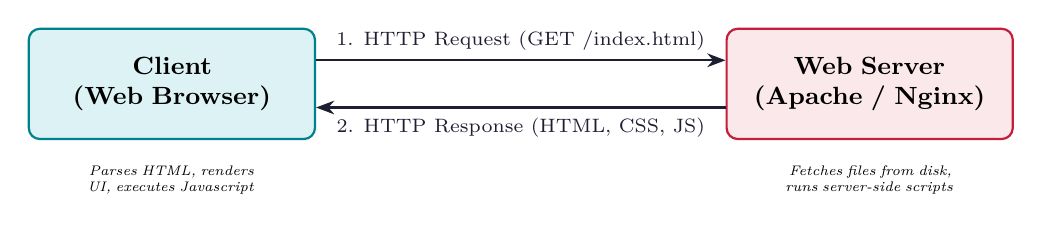
\begin{tikzpicture}[node distance=1.5cm and 5.2cm,
  browser/.style={rectangle, draw=myteal, fill=hdrteal, text width=3.4cm,
    align=center, minimum height=1.4cm, font=\small\bfseries, rounded corners=4pt, line width=0.8pt},
  server/.style={rectangle, draw=myred, fill=hdrred, text width=3.4cm,
    align=center, minimum height=1.4cm, font=\small\bfseries, rounded corners=4pt, line width=0.8pt}]

  % Nodes
  \node[browser] (client) {Client\\(Web Browser)};
  \node[server, right=of client] (server) {Web Server\\(Apache / Nginx)};

  % Paths
  \draw[arrow, transform canvas={yshift=0.3cm}] (client) -- (server) 
    node[midway, above, font=\scriptsize] {1. HTTP Request (GET /index.html)};
  \draw[arrow, transform canvas={yshift=-0.3cm}] (server) -- (client) 
    node[midway, below, font=\scriptsize] {2. HTTP Response (HTML, CSS, JS)};
    
  % Explanations
  \node[below=0.2cm of client, font=\tiny\itshape, text width=3.4cm, align=center] {Parses HTML, renders UI, executes Javascript};
  \node[below=0.2cm of server, font=\tiny\itshape, text width=3.4cm, align=center] {Fetches files from disk, runs server-side scripts};
\end{tikzpicture}
\end{tcolorbox}

\subsection{HTML vs. XML}
HTML and XML are both markup languages based on SGML, but they serve fundamentally different purposes:

\par\noindent
{\renewcommand{\arraystretch}{1.5}%
\begin{tabularx}{\linewidth}{|B{3.5cm}|Y|Y|}
\hline
\textbf{Feature} & \textbf{HTML (HyperText Markup Language)} & \textbf{XML (eXtensible Markup Language)} \\
\hline
\textbf{Primary Purpose} & Displaying and formatting data to users. & Transporting, storing, and structuring data. \\
\hline
\textbf{Tags} & Predefined tags (e.g., \texttt{<html>}, \texttt{<p>}). & Custom/user-defined tags based on data. \\
\hline
\textbf{Syntax Strictness} & Forgiving (errors don't crash rendering). & Extremely strict (well-formed check required). \\
\hline
\textbf{Case Sensitivity} & Case-insensitive (\texttt{<DIV>} and \texttt{<div>}). & Strictly case-sensitive. \\
\hline
\textbf{Closing Tags} & Optional for some tags (e.g., \texttt{<img>}, \texttt{<br>}). & Mandatory for all tags. \\
\hline
\end{tabularx}}

% ===============================================================================
\section{HTML Basics and Document Structure}
% ===============================================================================

\begin{tcolorbox}[defbox, title={\textbf{HTML --- HyperText Markup Language}}]
\textbf{HTML} is the standard markup language used to create the structure of web pages. It uses a set of hierarchical elements represented by tags to organize headings, paragraphs, tables, images, and other media elements.
\end{tcolorbox}

\subsection{Standard Skeleton of an HTML5 Document}
Every HTML document must follow a standard structural hierarchy:
\begin{spacing}{1.0}
\begin{verbatim}
<!DOCTYPE html>
<html>
  <head>
    <meta charset="UTF-8">
    <title>My Web Page</title>
  </head>
  <body>
    <h1>Welcome to Web Technology</h1>
    <p>This is a paragraph.</p>
  </body>
</html>
\end{verbatim}
\end{spacing}

\begin{tcolorbox}[tikzbox, title={HTML Document Object Model (DOM) Tree}]
\centering
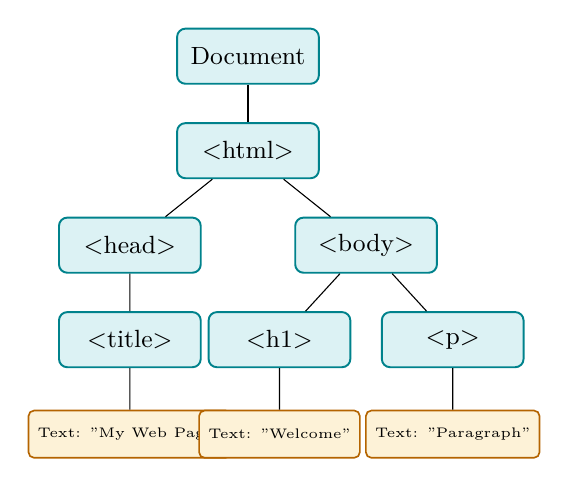
\begin{tikzpicture}[
  level 1/.style={sibling distance=5cm, level distance=1.2cm},
  level 2/.style={sibling distance=3cm, level distance=1.2cm},
  level 3/.style={sibling distance=2.2cm, level distance=1.2cm},
  node/.style={rectangle, draw=myteal, fill=hdrteal, minimum height=0.7cm, minimum width=1.8cm, font=\small, rounded corners=3pt, align=center, line width=0.7pt},
  textnode/.style={rectangle, draw=myamber, fill=hdramber, minimum height=0.6cm, minimum width=1.6cm, font=\tiny, rounded corners=2pt, align=center, line width=0.6pt}
]
  \node[node] {Document}
    child { node[node] {<html>}
      child { node[node] {<head>}
        child { node[node] {<title>}
          child { node[textnode] {Text: "My Web Page"} }
        }
      }
      child { node[node] {<body>}
        child { node[node] {<h1>}
          child { node[textnode] {Text: "Welcome"} }
        }
        child { node[node] {<p>}
          child { node[textnode] {Text: "Paragraph"} }
        }
      }
    };
\end{tikzpicture}
\end{tcolorbox}

\subsection{Block-level vs. Inline Elements}
HTML elements are categorized based on their default layout behaviors:

\par\noindent
{\renewcommand{\arraystretch}{1.5}%
\begin{tabularx}{\linewidth}{|B{3.2cm}|Y|Y|}
\hline
\textbf{Feature} & \textbf{Block-level Elements} & \textbf{Inline Elements} \\
\hline
\textbf{Layout Behavior} & Starts on a new line and takes up full width. & Stays on the same line and occupies only needed width. \\
\hline
\textbf{Margins \& Padding} & Fully respected on all four sides. & Top and bottom margins are ignored. \\
\hline
\textbf{Containment} & Can contain block or inline elements. & Can only contain inline elements / text. \\
\hline
\textbf{Examples} & \texttt{<div>, <p>, <h1>-<h6>, <ul>, <ol>, <table>} & \texttt{<span>, <a>, <strong>, <em>, <img>, <input>} \\
\hline
\end{tabularx}}

\subsection{Essential HTML Components}

\textbf{1. Lists:} HTML supports three list types:
\begin{itemize}[leftmargin=*, itemsep=3pt]
  \item \textbf{Unordered List (\texttt{<ul>}):} Bulleted list items using the \texttt{<li>} tag.
  \item \textbf{Ordered List (\texttt{<ol>}):} Numbered list items with customizable types (numeric, alphabetic, roman).
  \item \textbf{Description List (\texttt{<dl>}):} Pairs of terms (\texttt{<dt>}) and descriptions (\texttt{<dd>}).
\end{itemize}

\textbf{2. Links (Anchors \texttt{<a>}):} Used for navigating between pages or sections:
\begin{itemize}[leftmargin=*, itemsep=3pt]
  \item \textbf{Absolute Link:} Links to a fully qualified URL (e.g., \texttt{href="https://google.com"}).
  \item \textbf{Relative Link:} Links to a local resource relative to the file path (e.g., \texttt{href="about.html"}).
  \item \textbf{Email Link:} Triggers the client's email client using the mailto protocol (e.g., \texttt{href="mailto:test@test.com"}).
  \item \textbf{Anchor Targets:} Uses \texttt{target="\_blank"} to open in a new tab or \texttt{target="\_self"} for the same frame.
\end{itemize}

\textbf{3. Tables (\texttt{<table>}):} Formats data in rows and columns:
\begin{itemize}[leftmargin=*, itemsep=3pt]
  \item \textbf{Rowspan:} Extends a cell vertically across multiple rows (e.g., \texttt{<td rowspan="2">}).
  \item \textbf{Colspan:} Extends a cell horizontally across multiple columns (e.g., \texttt{<td colspan="3">}).
\end{itemize}

\textbf{4. Forms (\texttt{<form>}):} Captures and submits user inputs to a server. Key attributes:
\begin{itemize}[leftmargin=*, itemsep=3pt]
  \item \textbf{action:} The URL of the server-side endpoint that handles the submitted form data.
  \item \textbf{method:} The HTTP method used to send data (\texttt{GET} or \texttt{POST}).
  \item \textbf{Input Types:} Text, password, radio buttons, checkboxes, email, submit, file, number.
\end{itemize}

\textbf{5. Frames (\texttt{<frameset>}, \texttt{<frame>}, \texttt{<iframe>}):} Used to split the browser window into multiple independent document spaces:
\begin{itemize}[leftmargin=*, itemsep=3pt]
  \item \textbf{Traditional Frameset (\texttt{<frameset>}):} Replaces the \texttt{<body>} tag in HTML4 to partition the screen layout into rows or columns (e.g., \texttt{<frameset cols="25\%, 75\%">}). Each partition is defined using a \texttt{<frame src="...">} tag. \textit{Note: Deprecated in HTML5 due to poor accessibility, bookmarking difficulties, and bad SEO indexing.}
  \item \textbf{Inline Frames (\texttt{<iframe>}):} Used inside a standard \texttt{<body>} tag to embed another HTML page within the current page (e.g., \texttt{<iframe src="inner.html" width="300" height="200"></iframe>}). Widely used for embedding maps, videos, and third-party widgets.
\end{itemize}

% ===============================================================================
\section{CSS (Cascading Style Sheets)}
% ===============================================================================

\begin{tcolorbox}[defbox, title={\textbf{CSS --- Cascading Style Sheets}}]
\textbf{CSS} is a style sheet language used to describe the presentation, design, formatting, and layout of a document written in HTML. It separates structure from style, allowing consistent look-and-feel across multiple web pages.
\end{tcolorbox}

\subsection{Types of CSS Integration}

\par\noindent
{\renewcommand{\arraystretch}{1.5}%
\begin{tabularx}{\linewidth}{|B{3.0cm}|Y|Y|Y|}
\hline
\textbf{CSS Type} & \textbf{Syntax Example} & \textbf{Advantages} & \textbf{Disadvantages} \\
\hline
\textbf{Inline CSS} & \texttt{<p style="color:red;">} & High priority; quick overrides. & Messy; violates separation of concerns. \\
\hline
\textbf{Internal CSS} & \texttt{<style> p \{ color: red; \} </style>} & Contained inside single page; no extra HTTP request. & Reusability limit across multiple pages. \\
\hline
\textbf{External CSS} & \texttt{<link rel="stylesheet" href="style.css">} & High reuse; caching support; clean separation. & Requires extra network HTTP request. \\
\hline
\end{tabularx}}

\subsection{CSS Selectors}
CSS selectors target specific HTML elements for styling:
\begin{itemize}[leftmargin=*, itemsep=3pt]
  \item \textbf{Element Selector:} Targets all elements of a type (e.g., \texttt{p \{ color: red; \}}).
  \item \textbf{Class Selector:} Targets elements with a matching class name, preceded by a dot (e.g., \texttt{.container \{ width: 80\%; \}}).
  \item \textbf{ID Selector:} Targets a single element with a matching ID, preceded by a hash (e.g., \texttt{\#header \{ height: 60px; \}}). ID must be unique within the page.
  \item \textbf{Universal Selector:} Targets every element in the DOM using asterisk (e.g., \texttt{* \{ margin: 0; \}}).
\end{itemize}

\subsection{The CSS Box Model}
Every element in HTML is rendered as a rectangular box. The CSS Box Model defines how the size and spacing of this box are calculated.

\begin{tcolorbox}[tikzbox, title={CSS Box Model Layout}]
\centering
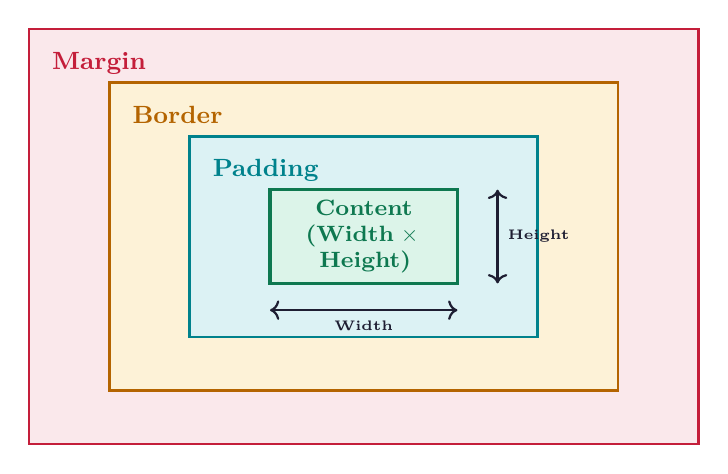
\begin{tikzpicture}[scale=0.85]
  % Outermost Margin
  \draw[line, fill=hdrred, draw=myred, line width=1pt] (0,0) rectangle (10,6.2);
  \node[anchor=north west, color=myred, font=\small\bfseries] at (0.2, 6.0) {Margin};

  % Border
  \draw[line, fill=hdramber, draw=myamber, line width=1pt] (1.2,0.8) rectangle (8.8,5.4);
  \node[anchor=north west, color=myamber, font=\small\bfseries] at (1.4, 5.2) {Border};

  % Padding
  \draw[line, fill=hdrteal, draw=myteal, line width=1pt] (2.4,1.6) rectangle (7.6,4.6);
  \node[anchor=north west, color=myteal, font=\small\bfseries] at (2.6, 4.4) {Padding};

  % Content
  \draw[line, fill=hdrgreen, draw=mygreen, line width=1.2pt] (3.6,2.4) rectangle (6.4,3.8);
  \node[color=mygreen, font=\footnotesize\bfseries, align=center, text width=2.4cm] at (5,3.1) {Content\\(Width $\times$ Height)};

  % Measurement markers
  \draw[arrow, <->, color=mydark] (3.6, 2.0) -- (6.4, 2.0) node[midway, below, font=\tiny\bfseries] {Width};
  \draw[arrow, <->, color=mydark] (7.0, 2.4) -- (7.0, 3.8) node[midway, right, font=\tiny\bfseries] {Height};
\end{tikzpicture}
\end{tcolorbox}

The dimensions of an element are computed based on the \texttt{box-sizing} property:
\begin{itemize}[leftmargin=*, itemsep=3pt]
  \item \textbf{\texttt{content-box} (Default):} Total Width = $\text{width} + \text{left/right padding} + \text{left/right border} + \text{left/right margin}$.
  \item \textbf{\texttt{border-box}:} Total Width = $\text{width} + \text{left/right margin}$ (padding and border are absorbed inside the specified width).
\end{itemize}

\newpage
% ===============================================================================
\begin{center}
  {\large\bfseries\color{myred} Quick Revision --- Module 1}\\[3pt]
  {\small\color{mydark} Web Development Basics (HTML \& CSS) $|$ OE-EC704A}
\end{center}
\noindent{\color{myred}\rule{\linewidth}{1.2pt}}
\vspace{4pt}

\begin{tcolorbox}[formulabox, title={\textbf{Core HTML Tags \& CSS Syntax}}]
{\renewcommand{\arraystretch}{1.3}%
\begin{tabularx}{\linewidth}{l Y}
\textbf{HTML Form / Tag} & \textbf{Syntax and Key Attributes} \\
\hline
Hyperlink Anchor & \texttt{<a href="URL" target="\_blank">Link Text</a>} \\
Embedded Image & \texttt{<img src="path" alt="Fallback text" width="500">} \\
HTML Table Structure & \texttt{<table> <tr> <td colspan="2">Data</td> </tr> </table>} \\
HTML Form Tag & \texttt{<form action="/login" method="POST"> inputs... </form>} \\
\hline
\textbf{CSS Selector Type} & \textbf{Syntax and Example Usage} \\
\hline
CSS Syntax Rule & \texttt{selector \{ property: value; \}} \\
Class Styling & \texttt{.button \{ background-color: blue; padding: 10px; \}} \\
ID Styling & \texttt{\#main-nav \{ display: flex; justify-content: space-between; \}} \\
Universal Reset & \texttt{* \{ box-sizing: border-box; margin: 0; padding: 0; \}} \\
\end{tabularx}}
\end{tcolorbox}

\begin{tcolorbox}[defbox, title={\textbf{One-Line Definitions}}]
\begin{itemize}[leftmargin=*, itemsep=2pt]
  \item \textbf{HTML:} Structured markup language defining content hierarchy of a web document.
  \item \textbf{CSS:} Style sheet language used for presenting and laying out HTML elements.
  \item \textbf{DOM (Document Object Model):} An API representing an HTML document as a logical tree structure.
  \item \textbf{Tag:} A code marker representing the start or end of an HTML element (e.g., \texttt{<p>}).
  \item \textbf{Element:} A complete component consisting of start tag, content, and end tag.
  \item \textbf{Attribute:} Name-value pairs inside HTML tags that modify their behavior or supply metadata.
  \item \textbf{Viewport:} The visible area of a web page on a client device screen.
  \item \textbf{URL (Uniform Resource Locator):} The global reference address of a web resource on the Internet.
\end{itemize}
\end{tcolorbox}

\begin{tcolorbox}[exambox, title={\textbf{Frequently Asked / Viva Questions}}]
\begin{enumerate}[leftmargin=*, label=\textbf{Q\arabic*.}, itemsep=5pt]
  \item \Q{What is the difference between \texttt{GET} and \texttt{POST} methods in forms?}
        \texttt{GET} appends form data directly to the URL as query parameters, rendering it visible and bookmarkable. It is intended for idempotent requests. \texttt{POST} sends data inside the HTTP message body, making it secure for sensitive parameters like passwords.
        
  \item \Q{Why is \texttt{DOCTYPE html} declared at the beginning of an HTML file?}
        It is a standard preamble instructing the client browser to render the document in standards-compliant mode rather than quirks mode.
        
  \item \Q{What is the difference between \texttt{span} and \texttt{div} tags?}
        \texttt{div} is a block-level container element that starts on a new line. \texttt{span} is an inline element used to style specific words or content inline without inserting page breaks.
        
  \item \Q{How does CSS specificity calculate which style to apply?}
        Specificity is calculated as a numeric weight: inline styles hold the highest priority (1000), followed by ID selectors (100), class/attribute selectors (10), and element selectors (1).
        
  \item \Q{What is the difference between relative and absolute positioning in CSS?}
        Relative positioning offsets an element relative to its normal position in the document flow. Absolute positioning moves the element relative to its closest parent with non-static positioning.
        
  \item \Q{What does the \texttt{box-sizing: border-box} property do?}
        It alters the CSS Box Model calculation so that borders and paddings are included in the element's declared width and height, preventing layout breakage.
        
  \item \Q{What are colspan and rowspan attributes in HTML tables?}
        \texttt{colspan} merges cells horizontally across columns. \texttt{rowspan} merges cells vertically across rows.
        
  \item \Q{What is semantic HTML and why is it important?}
        Semantic HTML uses tags that explain their purpose clearly (e.g., \texttt{<header>, <nav>, <article>, <footer>}) instead of generic \texttt{<div>} blocks. It enhances accessibility and SEO search indexing.
        
  \item \Q{How do you link CSS files to an HTML document?}
        Using the HTML \texttt{<link>} element inside the \texttt{<head>} block: \texttt{<link rel="stylesheet" href="style.css">}.
        
  \item \Q{What are CSS pseudoclasses and how are they used?}
        Pseudoclasses define special states of elements (e.g., \texttt{:hover} for mouse hover, \texttt{:active} for clicks, \texttt{:focus} for keyboard selection).
\end{enumerate}
\end{tcolorbox}

\begin{tcolorbox}[tikzbox, title={Form Submission: GET vs. POST comparison}]
\centering
{\renewcommand{\arraystretch}{1.45}%
\begin{tabularx}{\linewidth}{|B{3.2cm}|Y|Y|}
\hline
\textbf{Metric} & \textbf{GET Method} & \textbf{POST Method} \\
\hline
\textbf{Data Location} & Appended to URL (Query parameters). & Inside HTTP Request Body. \\
\hline
\textbf{Security} & Poor (exposed in browser history/logs). & Higher (hidden from URL path). \\
\hline
\textbf{Payload Limits} & Limited (typically ~2048 characters). & No architectural payload size limit. \\
\hline
\textbf{Caching} & Allowed/Cached by proxy servers. & Never cached. \\
\hline
\textbf{Idempotency} & Idempotent (submitting multiple times is safe). & Non-idempotent (resubmitting duplicates actions). \\
\hline
\end{tabularx}}
\end{tcolorbox}


% -- Module 2 -----------------------------------------------------------------
\modulestart{2}{Java Execution Environment}

\section{Java Execution Environment}
% ===============================================================================

Java uses a hybrid execution model combining compilation and interpretation. This ensures its core principle: \textbf{Write Once, Run Anywhere (WORA)}.

\begin{tcolorbox}[defbox, title={\textbf{Bytecode and Platform Independence}}]
\begin{itemize}[leftmargin=*, itemsep=3pt]
  \item \textbf{Bytecode:} A highly optimized set of machine instructions designed for execution by the JVM. It is stored in a \texttt{.class} file after compilation.
  \item \textbf{Platform Independence:} Java source code compiles into platform-independent bytecode. However, the \textbf{JVM itself is platform-dependent} because it must translate bytecode into the host system's native machine instructions.
\end{itemize}
\end{tcolorbox}

\begin{tcolorbox}[tikzbox, title={Java Compile-and-Run Execution Flow}]
\centering
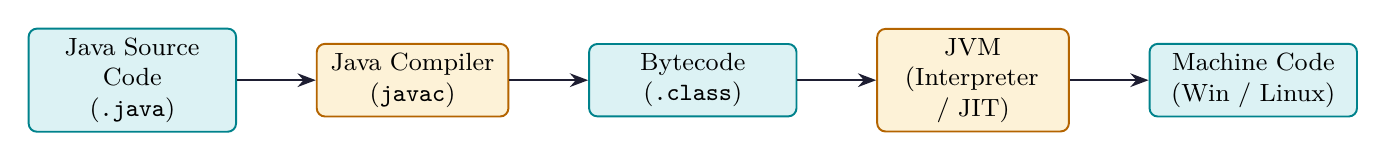
\begin{tikzpicture}[node distance=1.0cm and 1.8cm,
  node/.style={rectangle, draw=myteal, fill=hdrteal, text width=2.4cm,
    align=center, minimum height=0.9cm, font=\small, rounded corners=3pt, line width=0.7pt},
  act/.style={rectangle, draw=myamber, fill=hdramber, text width=2.2cm,
    align=center, minimum height=0.9cm, font=\small, rounded corners=3pt, line width=0.7pt}]

  % Nodes
  \node[node] (src) {Java Source Code\\(\texttt{.java})};
  \node[act, right=1.0cm of src] (compiler) {Java Compiler\\(\texttt{javac})};
  \node[node, right=1.0cm of compiler] (byte) {Bytecode\\(\texttt{.class})};
  \node[act, right=1.0cm of byte] (jvm) {JVM\\(Interpreter / JIT)};
  \node[node, right=1.0cm of jvm] (mach) {Machine Code\\(Win / Linux)};

  % Arrows
  \draw[arrow] (src) -- (compiler);
  \draw[arrow] (compiler) -- (byte);
  \draw[arrow] (byte) -- (jvm);
  \draw[arrow] (jvm) -- (mach);
\end{tikzpicture}
\end{tcolorbox}

\subsection{JDK vs. JRE vs. JVM}
Understanding the boundary between JVM, JRE, and JDK is crucial:

\begin{tcolorbox}[tikzbox, title={JDK, JRE, and JVM Containment Relationship}]
\centering
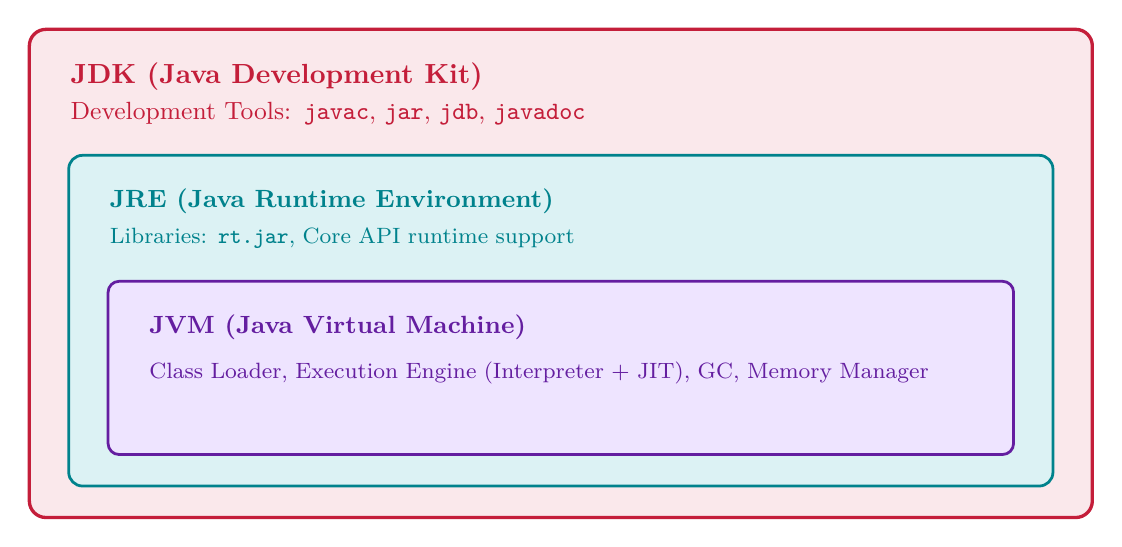
\begin{tikzpicture}
  % JDK Boundary
  \draw[draw=myred, fill=hdrred, line width=1.2pt, rounded corners=6pt] (0,0) rectangle (13.5,6.2);
  \node[anchor=north west, color=myred, font=\normalsize\bfseries] at (0.4, 5.9) {JDK (Java Development Kit)};
  \node[anchor=north west, color=myred, font=\small, align=left, text width=12.5cm] at (0.4, 5.4) {Development Tools: \texttt{javac}, \texttt{jar}, \texttt{jdb}, \texttt{javadoc}};

  % JRE Boundary
  \draw[draw=myteal, fill=hdrteal, line width=1.0pt, rounded corners=5pt] (0.5,0.4) rectangle (13.0,4.6);
  \node[anchor=north west, color=myteal, font=\small\bfseries] at (0.9, 4.3) {JRE (Java Runtime Environment)};
  \node[anchor=north west, color=myteal, font=\footnotesize, align=left, text width=11.5cm] at (0.9, 3.8) {Libraries: \texttt{rt.jar}, Core API runtime support};

  % JVM Boundary
  \draw[draw=mypurple, fill=hdrpurple, line width=1.0pt, rounded corners=4pt] (1.0,0.8) rectangle (12.5,3.0);
  \node[anchor=north west, color=mypurple, font=\small\bfseries] at (1.4, 2.7) {JVM (Java Virtual Machine)};
  \node[anchor=north west, color=mypurple, font=\footnotesize, align=left, text width=10.5cm] at (1.4, 2.1) {Class Loader, Execution Engine (Interpreter + JIT), GC, Memory Manager};
\end{tikzpicture}
\end{tcolorbox}

\par\noindent
{\renewcommand{\arraystretch}{1.5}%
\begin{tabularx}{\linewidth}{|B{3.2cm}|Y|Y|Y|}
\hline
\textbf{Metric} & \textbf{JVM (Virtual Machine)} & \textbf{JRE (Runtime)} & \textbf{JDK (Development)} \\
\hline
\textbf{Composition} & Classloader, Execution Engine, Garbage Collector. & JVM + Core class libraries (\texttt{rt.jar}) + plugins. & JRE + Compiler (\texttt{javac}) + tools (\texttt{jar}, \texttt{jdb}). \\
\hline
\textbf{Purpose} & Execution of compiled bytecode. & Running Java applications. & Developing and running Java apps. \\
\hline
\textbf{Target User} & None (internal engine). & End users/clients. & Developers. \\
\hline
\end{tabularx}}

% ===============================================================================
\section{Java Characteristics and Features}
% ===============================================================================

Java's design is guided by a set of primary characteristics (often called "Java Buzzwords"):

\begin{tcolorbox}[defbox, title={\textbf{Core Java Characteristics}}]
\begin{enumerate}[leftmargin=*, itemsep=3pt]
  \item \textbf{Simple:} Clean syntax derived from C++ but without complex features like pointers, operator overloading, or multiple inheritance.
  \item \textbf{Object-Oriented:} Everything in Java is an object (except primitive types), promoting modularity and extensibility.
  \item \textbf{Robust:} Emphasizes early error checking via compile-time checking, runtime exception handling, and automatic garbage collection.
  \item \textbf{Secure:} Executes inside a virtual machine sandbox without direct memory manipulation or pointers, preventing buffer overflows and unauthorized system access.
  \item \textbf{Portable and Architecture-Neutral:} Compiles to bytecode that can run on any device with a compatible JVM, without needing recompilation.
  \item \textbf{Multithreaded:} Built-in support for concurrent execution of multiple tasks, improving resource utilization in GUI and server applications.
\end{enumerate}
\end{tcolorbox}
% ===============================================================================
\section{Object-Oriented Programming (OOP) Concepts}
% ===============================================================================

Object-Oriented Programming (OOP) is a programming paradigm based on the concept of "objects," which can contain data (in the form of fields or attributes) and code (in the form of procedures or methods). Java is a class-based, object-oriented language.

\begin{tcolorbox}[defbox, title={\textbf{Class vs. Object}}]
\begin{itemize}[leftmargin=*, itemsep=3pt]
  \item \textbf{Class:} A logical blueprint or template used to create objects. It defines the state (attributes) and behavior (methods) that all objects of this class will share. It does not occupy memory space.
  \item \textbf{Object:} A physical instance of a class. It has state, behavior, and a unique identity. It occupies physical memory space on the heap.
\end{itemize}
\end{tcolorbox}

\subsection{The Four Pillars of OOP}
Java fully implements the four core principles of object-oriented programming:

\begin{enumerate}[leftmargin=*, itemsep=6pt]
  \item \textbf{Encapsulation (Data Hiding):}
        The process of wrapping data (variables) and code (methods) together as a single unit (class) while restricting direct access to the state.
        \begin{itemize}[leftmargin=*, label=--]
          \item \textbf{Implementation:} Declare instance variables as \texttt{private} and provide access via public getter and setter methods.
          \item \textbf{Advantage:} Provides security, data validation, and flexibility to make variables read-only or write-only.
        \end{itemize}
  \item \textbf{Abstraction (Implementation Hiding):}
        Hiding internal implementation details and exposing only the essential features of an object.
        \begin{itemize}[leftmargin=*, label=--]
          \item \textbf{Implementation:} Achieved via \texttt{abstract} classes and \texttt{interfaces}.
          \item \textbf{Advantage:} Reduces complexity and isolates the user from implementation changes.
        \end{itemize}
  \item \textbf{Inheritance (Code Reusability):}
        The mechanism by which one class (subclass) inherits the fields and methods of another class (superclass).
        \begin{itemize}[leftmargin=*, label=--]
          \item \textbf{Implementation:} Achieved using the \texttt{extends} keyword. Java supports single, multilevel, and hierarchical inheritance but does not support multiple inheritance with classes to avoid ambiguity (the "Diamond Problem").
          \item \textbf{Advantage:} Promotes code reusability and establishes an "IS-A" relationship.
        \end{itemize}
  \item \textbf{Polymorphism (Many Forms):}
        The ability of a single action, method, or object to behave differently depending on the context.
        \begin{itemize}[leftmargin=*, label=--]
          \item \textbf{Compile-time (Static) Polymorphism:} Resolved during compilation. Achieved via \textbf{Method Overloading} (same method name, different parameters).
          \item \textbf{Runtime (Dynamic) Polymorphism:} Resolved during runtime. Achieved via \textbf{Method Overriding} (same method name and signature in subclass) and \textbf{Dynamic Method Dispatch}.
        \end{itemize}
\end{enumerate}

\begin{tcolorbox}[tikzbox, title={The Four Pillars of OOP}]
\centering
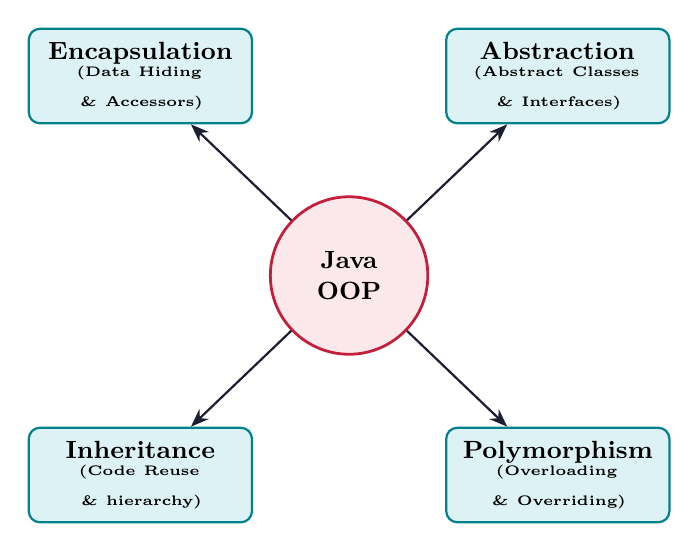
\begin{tikzpicture}[node distance=1.0cm and 0.8cm,
  pillar/.style={rectangle, draw=myteal, fill=hdrteal, text width=2.6cm,
    align=center, minimum height=1.2cm, font=\small\bfseries, rounded corners=4pt, line width=0.8pt},
  core/.style={circle, draw=myred, fill=hdrred, minimum size=2.0cm,
    align=center, font=\small\bfseries, line width=1.0pt}]

  % Central Core
  \node[core] (oop) {Java\\OOP};

  % Pillars
  \node[pillar, above left=1.2cm and 0.5cm of oop] (enc) {Encapsulation\\{\tiny (Data Hiding\\\& Accessors)}};
  \node[pillar, above right=1.2cm and 0.5cm of oop] (abs) {Abstraction\\{\tiny (Abstract Classes\\\& Interfaces)}};
  \node[pillar, below left=1.2cm and 0.5cm of oop] (inh) {Inheritance\\{\tiny (Code Reuse\\\& hierarchy)}};
  \node[pillar, below right=1.2cm and 0.5cm of oop] (poly) {Polymorphism\\{\tiny (Overloading\\\& Overriding)}};

  % Arrows
  \draw[arrow] (oop) -- (enc);
  \draw[arrow] (oop) -- (abs);
  \draw[arrow] (oop) -- (inh);
  \draw[arrow] (oop) -- (poly);
\end{tikzpicture}
\tcbset{after={\color{black}}}
\end{tcolorbox}

% ===============================================================================
\section{Structure of a Simple Java Program}
% ===============================================================================

Every standard standalone Java application has an entry point class containing a main method.

\subsection{Standard Hello World Program}
Below is a simple Java program that prints a message to the console:
\begin{verbatim}
public class HelloWorld {
    // Execution entry point
    public static void main(String[] args) {
        System.out.println("Hello, World!");
    }
}
\end{verbatim}

\subsection{Key Elements Explained}
\begin{itemize}[leftmargin=*, itemsep=4pt]
  \item \textbf{\texttt{public class HelloWorld}:} Declares a public class named \texttt{HelloWorld}. In Java, the file name must match the name of the public class it contains (e.g., \texttt{HelloWorld.java}).
  \item \textbf{\texttt{public static void main(String[] args)}:} The entry point of the program:
        \begin{itemize}[leftmargin=*, label=--]
          \item \textbf{\texttt{public}:} Accessible by the JVM from outside the class.
          \item \textbf{\texttt{static}:} Can be called without creating an instance of the class.
          \item \textbf{\texttt{void}:} Returns no value to the runtime environment.
          \item \textbf{\texttt{String[] args}:} Array of command-line arguments passed as strings.
        \end{itemize}
  \item \textbf{\texttt{System.out.println()}:} Built-in output stream to print text followed by a new line to the console.
\end{itemize}

\subsection{Compiling and Running Java Programs}
Java programs require a two-step compile-and-run sequence:
\begin{enumerate}[leftmargin=*, itemsep=3.5pt]
  \item \textbf{Compilation:} Run the compiler (\texttt{javac}) to convert the source code into bytecode class files:
        \begin{verbatim}
        javac HelloWorld.java
        \end{verbatim}
        This generates a file named \texttt{HelloWorld.class} containing platform-independent bytecode.
  \item \textbf{Execution:} Run the JVM interpreter (\texttt{java}) to load and execute the class file:
        \begin{verbatim}
        java HelloWorld
        \end{verbatim}
        (Note: Do not include the \texttt{.class} extension when executing the program).
\end{enumerate}

% ===============================================================================
\section{Data Types, Operators, and Expressions}
% ===============================================================================

\subsection{Primitive vs. Reference Data Types}
Java enforces static type checking and groups types into two primary categories:

\par\noindent
{\renewcommand{\arraystretch}{1.5}%
\begin{tabularx}{\linewidth}{|B{3.2cm}|Y|Y|}
\hline
\textbf{Feature} & \textbf{Primitive Data Types} & \textbf{Reference Data Types} \\
\hline
\textbf{Allocation} & Stored directly on the stack memory. & Object on Heap; address reference on Stack. \\
\hline
\textbf{Default Value} & \texttt{0}, \texttt{0.0}, or \texttt{false} (never null). & \texttt{null} by default. \\
\hline
\textbf{Size} & Fixed sizing (e.g., \texttt{int}: 32-bit, \texttt{double}: 64-bit). & Depends on the host system architecture. \\
\hline
\textbf{Examples} & \texttt{byte, short, int, long, float, double, char, boolean} & Classes, interfaces, arrays, strings. \\
\hline
\end{tabularx}}

\subsection{Memory Allocation Model}
Java allocates memory across two distinct spaces during runtime:
\begin{itemize}[leftmargin=*, itemsep=3pt]
  \item \textbf{Stack Memory:} Stores primitive variables and local references. Uses LIFO (Last In First Out) allocation.
  \item \textbf{Heap Memory:} Dynamic memory pool that hosts all runtime objects and instance variables.
\end{itemize}

\begin{tcolorbox}[tikzbox, title={Stack and Heap Memory Layout}]
\centering
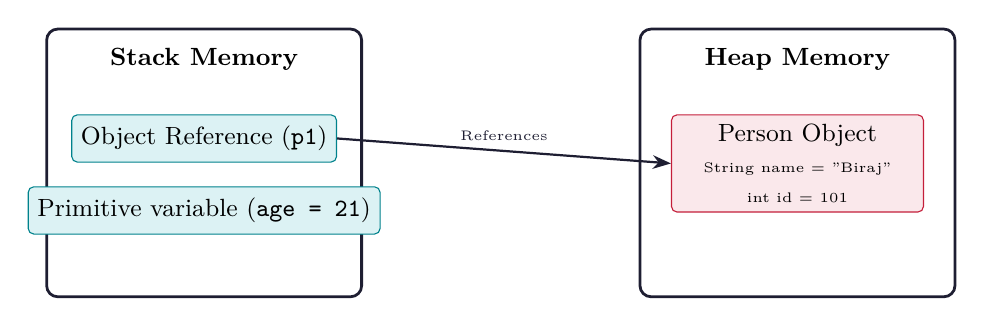
\begin{tikzpicture}[node distance=1.5cm,
  space/.style={rectangle, draw=mydark, line width=1pt, minimum width=4cm, minimum height=3.4cm, rounded corners=4pt},
  element/.style={rectangle, draw=myteal, fill=hdrteal, minimum width=3.2cm, minimum height=0.6cm, font=\small, rounded corners=2pt}]

  % Stack Frame
  \node[space] (stack) {};
  \node[anchor=north, font=\small\bfseries, yshift=-4pt] at (stack.north) {Stack Memory};
  \node[element, below=1.1cm of stack.north] (ref) {Object Reference (\texttt{p1})};
  \node[element, below=0.3cm of ref] (age) {Primitive variable (\texttt{age = 21})};

  % Heap Frame
  \node[space, right=3.5cm of stack] (heap) {};
  \node[anchor=north, font=\small\bfseries, yshift=-4pt] at (heap.north) {Heap Memory};
  \node[rectangle, draw=myred, fill=hdrred, minimum width=3.2cm, minimum height=1.2cm, rounded corners=2pt, below=1.1cm of heap.north, font=\small, align=center] (obj) {Person Object\\{\tiny String name = "Biraj"}\\{\tiny int id = 101}};

  % Connection
  \draw[arrow] (ref.east) -- (obj.west) node[midway, above, font=\tiny] {References};
\end{tikzpicture}
\end{tcolorbox}

\subsection{Operators and Expressions}
Java provides a comprehensive set of operators to build computational expressions:
\begin{itemize}[leftmargin=*, itemsep=3pt]
  \item \textbf{Arithmetic Operators:} Binary (\texttt{+}, \texttt{-}, \texttt{*}, \texttt{/}, \texttt{\%}) and Unary (\texttt{++}, \texttt{--}).
  \item \textbf{Relational Operators:} Compare operands for equality or order (\texttt{==}, \texttt{!=}, \texttt{<}, \texttt{>}, \texttt{<=}, \texttt{>=}).
  \item \textbf{Logical Operators:} Combine boolean expressions (\texttt{\&\&} (logical AND), \texttt{||} (logical OR), \texttt{!} (logical NOT)). Supports short-circuit evaluation.
  \item \textbf{Bitwise Operators:} Perform bit-level manipulations (\texttt{\&}, \texttt{|}, \texttt{\^}, \texttt{\~}, \texttt{<<}, \texttt{>>}, \texttt{>>>}).
  \item \textbf{Ternary Operator:} Conditional assignment shorthand (\texttt{variable = (condition) ? valueIfTrue : valueIfFalse}).
\end{itemize}

% ===============================================================================
\section{Control Flow and Branching}
% ===============================================================================

Java supports selection, iteration, and jump statements to control execution paths:
\begin{itemize}[leftmargin=*, itemsep=4pt]
  \item \textbf{Selection Statements:} \texttt{if-else} blocks for boolean conditions and \texttt{switch} blocks for multi-way branching (supports byte, short, char, int, Enums, and String).
  \item \textbf{Iteration Statements:} 
        \begin{itemize}[leftmargin=*, label=--]
          \item \texttt{for} loops for index-based loops.
          \item \texttt{while} loops for condition-controlled loops (pre-test).
          \item \texttt{do-while} loops for exit-controlled loops (post-test, runs at least once).
        \end{itemize}
  \item \textbf{Jump Statements:}
        \begin{itemize}[leftmargin=*, label=--]
          \item \texttt{break}: Terminated loop or switch block immediately.
          \item \texttt{continue}: Skips the rest of the current loop body and proceeds to the next iteration step.
          \item Labeled Statements: Loops can be labeled (e.g., \texttt{outerLoop: for(...)}) to specify which loop a nested \texttt{break} or \texttt{continue} targets.
        \end{itemize}
\end{itemize}

\newpage
% ===============================================================================
\begin{center}
  {\large\bfseries\color{myred} Quick Revision --- Module 2}\\[3pt]
  {\small\color{mydark} Introduction to Java Programming \& OOP $|$ OE-EC704A}
\end{center}
\noindent{\color{myred}\rule{\linewidth}{1.2pt}}
\vspace{4pt}

\begin{tcolorbox}[formulabox, title={\textbf{Java Basic Syntax \& Loop Structures}}]
{\renewcommand{\arraystretch}{1.3}%
\begin{tabularx}{\linewidth}{l Y}
\textbf{Concept} & \textbf{Syntax and Example Usage} \\
\hline
Simple Program & \texttt{public class Test \{ public static void main(String[] args) \{ ... \} \}} \\
Data Type Sizing & \texttt{byte} (8-bit), \texttt{char} (16-bit Unicode), \texttt{int} (32-bit), \texttt{double} (64-bit) \\
Ternary Operator & \texttt{int min = (a < b) ? a : b;} \\
Short-Circuit logic & \texttt{if (obj != null \&\& obj.isValid()) \{ ... \} // prevents NPE} \\
\hline
\textbf{Loop Statements} & \textbf{Conditional and Iterative Formats} \\
\hline
\texttt{for} Loop & \texttt{for(int i = 0; i < n; i++) \{ ... \}} \\
\texttt{while} Loop & \texttt{while(condition) \{ statements; \}} \\
\texttt{do-while} Loop & \texttt{do \{ statements; \} while(condition);} \\
Labeled Break & \texttt{outer: for(...) \{ if(cond) break outer; \}} \\
\end{tabularx}}
\end{tcolorbox}

\begin{tcolorbox}[defbox, title={\textbf{One-Line Definitions}}]
\begin{itemize}[leftmargin=*, itemsep=2pt]
  \item \textbf{JVM (Java Virtual Machine):} The abstract execution engine that interprets and executes compiled Java bytecode.
  \item \textbf{Bytecode:} Platform-independent intermediate code representation generated by \texttt{javac}.
  \item \textbf{JDK:} Java Development Kit containing compiler, tools, and the JRE runtime.
  \item \textbf{JRE:} Java Runtime Environment providing JVM and core system class libraries.
  \item \textbf{Stack Memory:} LIFO memory space storing local variables and function execution frames.
  \item \textbf{Heap Memory:} General dynamic memory pool where all Java objects are instantiated.
  \item \textbf{Short-Circuiting:} Logical expression evaluation that stops as soon as the outcome is guaranteed.
  \item \textbf{Platform Independence:} The ability of bytecode to run unmodified on any OS running a JVM.
  \item \textbf{Encapsulation:} Wrapping variables and methods into a class and restricting direct access.
  \item \textbf{Abstraction:} Hiding execution details and exposing only the interface contract.
  \item \textbf{Inheritance:} Class relationship mechanism enabling child reuse of parent methods/variables.
  \item \textbf{Polymorphism:} Feature allowing a single entity to assume different behaviors at runtime or compile-time.
\end{itemize}
\tcbset{after={\color{black}}}
\end{tcolorbox}

\begin{tcolorbox}[exambox, title={\textbf{Frequently Asked / Viva Questions}}]
\begin{enumerate}[leftmargin=*, label=\textbf{Q\arabic*.}, itemsep=5pt]
  \item \Q{Why is Java platform-independent but JVM is platform-dependent?}
        Java bytecode is standardized and can run on any machine. However, the JVM must be custom-tailored to the target operating system to translate that bytecode to native CPU instructions.
        
  \item \Q{What is JIT Compiler in Java?}
        The Just-In-Time (JIT) compiler is a component of the JVM execution engine. It compiles frequently executed bytecode (hot spots) directly into native machine code at runtime to boost performance.
        
  \item \Q{What is the difference between \texttt{path} and \texttt{classpath} variables?}
        \texttt{path} is an OS environment variable that locates shell commands like \texttt{javac} and \texttt{java}. \texttt{classpath} is a JVM-specific setting directing the classloader where to find compiled user class files.
        
  \item \Q{What are the JVM memory partitions?}
        JVM memory is divided into: Method Area (class metadata, static variables), Heap (objects), Stack (local variables, execution frames), PC Register (current instruction address), and Native Method Stack.
        
  \item \Q{Why does Java use Unicode for characters?}
        Java was designed for global applications. While ASCII uses 8 bits and represents 256 characters, Unicode uses 16 bits, allowing it to represent characters from all major languages.
        
  \item \Q{What is the difference between prefix and postfix increment operators?}
        Prefix (\texttt{++i}) increments the variable first and then returns the incremented value. Postfix (\texttt{i++}) returns the original value first and then increments the variable.
        
  \item \Q{Explain short-circuit logical operators.}
        In \texttt{A \&\& B}, if \texttt{A} is false, the JVM skips evaluating \texttt{B} since the result is guaranteed to be false. Similarly, in \texttt{A || B}, if \texttt{A} is true, \texttt{B} is not evaluated.
        
  \item \Q{Can we use a String in a switch-case statement?}
        Yes, starting from Java 7, String literals are supported in switch-case statements. The JVM compares strings using their \texttt{equals()} values and hash codes.
        
  \item \Q{What is the difference between \texttt{break} and \texttt{continue} statements?}
        \texttt{break} terminates the loop completely, passing control to the statement after the loop. \texttt{continue} terminates only the current loop iteration, jumping to the loop update/condition.
        
  \item \Q{Why is there no \texttt{goto} statement in Java?}
        Java does not support \texttt{goto} to enforce clean structured programming principles and prevent "spaghetti code." Instead, labeled break and continue statements are provided.
        
  \item \Q{Explain the four pillars of OOP and their implementation in Java.}
        The four pillars are: Abstraction (hiding implementation details via abstract classes and interfaces), Encapsulation (data hiding using private attributes and public getters/setters), Inheritance (code reuse using subclassing with the \texttt{extends} keyword), and Polymorphism (methods behaving differently based on context via method overloading and overriding).
        
  \item \Q{Why is the main method in Java declared as \texttt{public static void}?}
        \texttt{public} makes it accessible to the JVM from outside the class context. \texttt{static} allows the JVM to execute the method without instantiating the class first. \texttt{void} specifies that it returns no value to the operating system after execution completes.
\end{enumerate}
\end{tcolorbox}

\begin{tcolorbox}[tikzbox, title={Java Iteration Statement Comparisons}]
\centering
{\renewcommand{\arraystretch}{1.45}%
\begin{tabularx}{\linewidth}{|B{2.8cm}|Y|Y|Y|}
\hline
\textbf{Feature} & \textbf{\texttt{for} Loop} & \textbf{\texttt{while} Loop} & \textbf{\texttt{do-while} Loop} \\
\hline
\textbf{Loop Structure} & Counter-based iteration. & Condition-controlled iteration. & Exit-controlled iteration. \\
\hline
\textbf{Condition Check} & Evaluated at start. & Evaluated at start. & Evaluated at end. \\
\hline
\textbf{Min. Runs} & 0 runs if condition fails. & 0 runs if condition fails. & Guaranteed at least 1 run. \\
\hline
\textbf{Best Use Case} & Iterating when count is known. & Loop until event triggers. & Interactive menus. \\
\hline
\end{tabularx}}
\end{tcolorbox}


% -- Module 3 -----------------------------------------------------------------
\modulestart{3}{Class Fundamentals and Objects}

\section{Class Fundamentals and Objects}
% ===============================================================================

In Java, all program logic resides within classes. A class acts as a blueprint, and objects are active physical instances of that blueprint.

\begin{tcolorbox}[defbox, title={\textbf{Class Declaration \& Object Creation}}]
\begin{itemize}[leftmargin=*, itemsep=3pt]
  \item \textbf{Declaring a Class:} Declared using the \texttt{class} keyword. It encapsulates state (instance variables) and behavior (methods).
  \item \textbf{Creating Instances:} Objects are created dynamically on the heap using the \texttt{new} keyword, which allocates memory and invokes the constructor.
\end{itemize}
\end{tcolorbox}

\begin{tcolorbox}[tikzbox, title={Object Creation and Reference Linkage}]
\centering
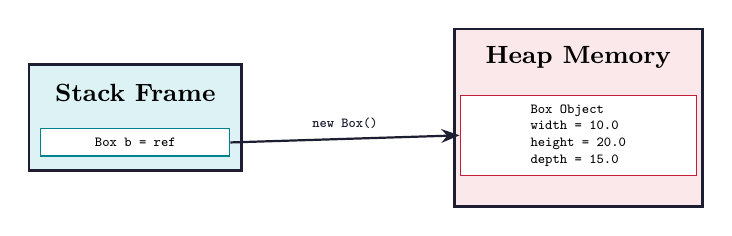
\begin{tikzpicture}[scale=0.9]
  % Stack Side
  \draw[draw=mydark, fill=hdrteal, line width=1pt] (-4,0) rectangle (-1,1.5);
  \node at (-2.5, 1.1) {\small\bfseries Stack Frame};
  \node[draw=myteal, fill=white, font=\tiny\ttfamily, minimum width=2.4cm] (var) at (-2.5, 0.4) {Box b = ref};

  % Heap Side
  \draw[draw=mydark, fill=hdrred, line width=1pt] (2,-0.5) rectangle (5.5,2);
  \node at (3.75, 1.6) {\small\bfseries Heap Memory};
  \node[draw=myred, fill=white, font=\tiny\ttfamily, align=left, minimum width=3cm] (obj) at (3.75, 0.5) {Box Object\\width = 10.0\\height = 20.0\\depth = 15.0};

  % Arrow
  \draw[arrow] (var.east) -- (obj.west) node[midway, above, font=\tiny\bfseries] {\texttt{new Box()}};
\end{tikzpicture}
\end{tcolorbox}

\subsection{Constructors in Java}
A constructor initializes the state of a newly created object. It has no return type and must have the same name as the class.

\begin{itemize}[leftmargin=*, itemsep=4pt]
  \item \textbf{Default Constructor:} Automatically provided by the compiler if no explicit constructor is defined. It initializes primitives to their default values (e.g., \texttt{0}, \texttt{false}) and object references to \texttt{null}.
  \item \textbf{Parameterized Constructor:} User-defined constructor that accepts parameters to initialize instances with custom values.
  \item \textbf{Copy Constructor:} A constructor that initializes a new object using an existing object of the same class:
        \begin{verbatim}
        class Box {
            double width, height;
            Box(Box ob) { // Copy Constructor
                this.width = ob.width;
                this.height = ob.height;
            }
        }
        \end{verbatim}
\end{itemize}

\subsection{Argument Passing in Java}
Java uses a single parameter passing mechanism: \textbf{Pass-by-Value}.
\begin{itemize}[leftmargin=*, itemsep=3.5pt]
  \item \textbf{Primitive Arguments:} A copy of the value is passed. Changes made inside the method do not affect the original variable.
  \item \textbf{Object Arguments:} A copy of the reference address is passed. The method can modify the object's contents (since they both point to the same object on the heap), but reassigning the reference variable inside the method does not affect the caller's original reference.
\end{itemize}

\subsection{The \texttt{static} Keyword}
The \texttt{static} keyword is used to create class-level members that are shared across all instances.
\begin{itemize}[leftmargin=*, itemsep=4pt]
  \item \textbf{Static Variables:} Single memory copy allocated in the method area, shared by all objects of that class.
  \item \textbf{Static Methods:} Methods that can be called without creating an instance. They can only access static data and call other static methods. They cannot use the \texttt{this} or \texttt{super} keywords.
  \item \textbf{Static Blocks:} Used to initialize static variables. Executed automatically when the class is first loaded into memory, before the main method or object constructors.
\end{itemize}

\subsection{Nested and Inner Classes}
Java allows defining a class inside another class.
\begin{itemize}[leftmargin=*, itemsep=4pt]
  \item \textbf{Member Inner Class:} A non-static class declared inside another. It has access to all members (including private ones) of the outer class. It requires an instance of the outer class to exist.
  \item \textbf{Static Nested Class:} Declared static. It behaves like a top-level class packaged inside another class. It cannot access non-static outer members.
  \item \textbf{Local Inner Class:} Defined inside a block or method. It can only access local variables if they are effectively final.
  \item \textbf{Anonymous Inner Class:} An inner class defined inline without a name, typically used for overriding listener methods or implementing interfaces on the fly.
\end{itemize}

% ===============================================================================
\section{Inheritance and Reuse Models}
% ===============================================================================

Inheritance enables hierarchical classifications. In Java, classes are extended using the \texttt{extends} keyword.

\begin{tcolorbox}[defbox, title={\textbf{Inheritance Characteristics}}]
\begin{itemize}[leftmargin=*, itemsep=3pt]
  \item \textbf{Single Inheritance Only:} Java classes can only extend \textbf{one} parent class to prevent the diamond problem (ambiguity under duplicate variable/method signatures).
  \item \textbf{The \texttt{super} Keyword:} Used to invoke the parent class constructor (must be the first statement in the subclass constructor), access overridden parent methods, or read hidden parent variables.
\end{itemize}
\end{tcolorbox}

\begin{tcolorbox}[tikzbox, title={Inheritance Trees supported in Java}]
\centering
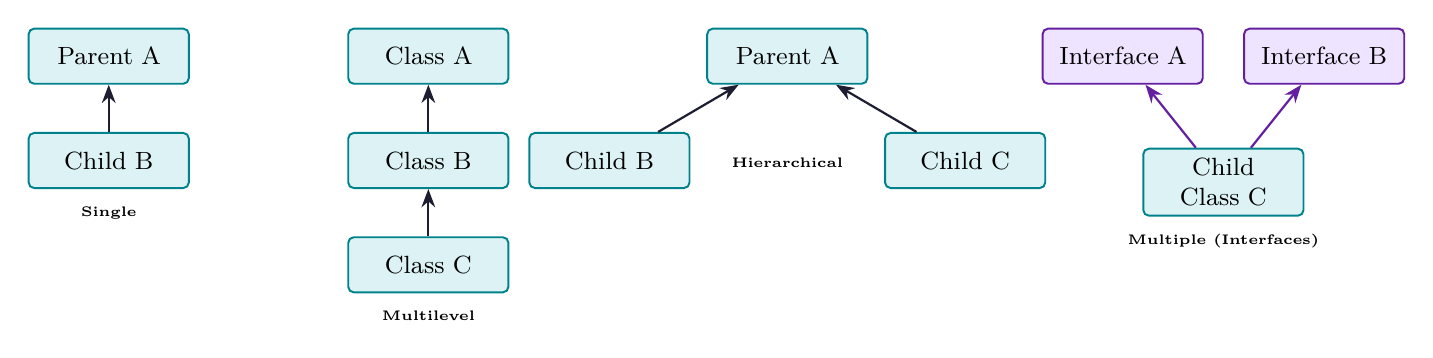
\begin{tikzpicture}[node distance=1.0cm and 1.8cm,
  cls/.style={rectangle, draw=myteal, fill=hdrteal, text width=1.8cm,
    align=center, minimum height=0.7cm, font=\small, rounded corners=2pt, line width=0.7pt},
  intf/.style={rectangle, draw=mypurple, fill=hdrpurple, text width=1.8cm,
    align=center, minimum height=0.7cm, font=\small, rounded corners=2pt, line width=0.7pt}]

  % --- Single ---
  \node[cls] (S1) {Parent A};
  \node[cls, below=0.6cm of S1] (S2) {Child B};
  \draw[arrow] (S2) -- (S1);
  \node[below=0.1cm of S2, font=\tiny\bfseries] {Single};

  % --- Multilevel ---
  \node[cls, right=2.0cm of S1] (M1) {Class A};
  \node[cls, below=0.6cm of M1] (M2) {Class B};
  \node[cls, below=0.6cm of M2] (M3) {Class C};
  \draw[arrow] (M3) -- (M2);
  \draw[arrow] (M2) -- (M1);
  \node[below=0.1cm of M3, font=\tiny\bfseries] {Multilevel};

  % --- Hierarchical ---
  \node[cls, right=2.5cm of M1] (H1) {Parent A};
  \node[cls, below left=0.6cm and 0.2cm of H1] (H2) {Child B};
  \node[cls, below right=0.6cm and 0.2cm of H1] (H3) {Child C};
  \draw[arrow] (H2) -- (H1);
  \draw[arrow] (H3) -- (H1);
  \node[below=0.8cm of H1, font=\tiny\bfseries] {Hierarchical};

  % --- Multiple (via Interfaces) ---
  \node[intf, right=2.2cm of H1] (I1) {Interface A};
  \node[intf, right=0.5cm of I1] (I2) {Interface B};
  \node[cls, below=0.8cm of $(I1.south)!0.5!(I2.south)$] (I3) {Child Class C};
  \draw[arrow, color=mypurple] (I3) -- (I1);
  \draw[arrow, color=mypurple] (I3) -- (I2);
  \node[below=0.1cm of I3, font=\tiny\bfseries] {Multiple (Interfaces)};
\end{tikzpicture}
\end{tcolorbox}

\subsection{Composition vs. Inheritance}
Design patterns advocate favoring object composition over class inheritance:

\par\noindent
{\renewcommand{\arraystretch}{1.5}%
\begin{tabularx}{\linewidth}{|B{3.2cm}|Y|Y|}
\hline
\textbf{Metric} & \textbf{Composition (Has-A Relationship)} & \textbf{Inheritance (Is-A Relationship)} \\
\hline
\textbf{Coupling Level} & Loose coupling; internal details remain private. & Tight coupling; breaks encapsulation boundary. \\
\hline
\textbf{Flexibility} & Behaviors can change dynamically at runtime. & Static; behavior fixed at compilation time. \\
\hline
\textbf{Design Reuse} & Reuses functional components as class members. & Reuses code by expanding a class hierarchy. \\
\hline
\textbf{Example} & \texttt{Car} has an \texttt{Engine} instance. & \texttt{Car} is a subclass of \texttt{Vehicle}. \\
\hline
\end{tabularx}}

% ===============================================================================
\section{Polymorphism and Runtime Resolution}
% ===============================================================================

\subsection{Method Overloading vs. Overriding}
These represent static and dynamic polymorphism:

\par\noindent
{\renewcommand{\arraystretch}{1.5}%
\begin{tabularx}{\linewidth}{|B{3.0cm}|Y|Y|}
\hline
\textbf{Feature} & \textbf{Method Overloading (Static)} & \textbf{Method Overriding (Dynamic)} \\
\hline
\textbf{Class Context} & Occurs within the same class definition. & Occurs across child-parent subclass hierarchy. \\
\hline
\textbf{Method Signature} & Name must be same; parameters must differ. & Signature (parameters, returns) must match. \\
\hline
\textbf{Resolution Time} & Compile-time (static binding). & Runtime (dynamic binding). \\
\hline
\textbf{Keywords} & None required. & Assisted by \texttt{@Override} annotation. \\
\hline
\end{tabularx}}

\subsection{Dynamic Method Dispatch}
Dynamic Method Dispatch is the mechanism by which a call to an overridden method is resolved at runtime rather than compile-time.

\begin{tcolorbox}[defbox, title={\textbf{Dynamic Method Dispatch Rule}}]
When an overridden method is called through a superclass reference, Java determines which version of the method to execute based on the \textbf{type of the actual object} being referred to at runtime, not the type of the reference variable.
\end{tcolorbox}

\begin{tcolorbox}[tikzbox, title={Dynamic Method Dispatch Flow}]
\centering
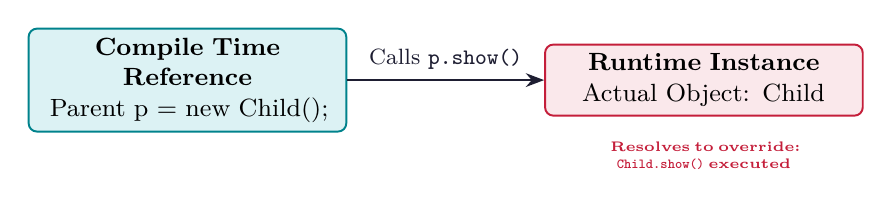
\begin{tikzpicture}[node distance=1.5cm and 2.5cm,
  refnode/.style={rectangle, draw=myteal, fill=hdrteal, text width=3.8cm,
    align=center, minimum height=0.8cm, font=\small, rounded corners=3pt, line width=0.7pt},
  instnode/.style={rectangle, draw=myred, fill=hdrred, text width=3.8cm,
    align=center, minimum height=0.8cm, font=\small, rounded corners=3pt, line width=0.7pt}]

  % Compilation (Reference Type)
  \node[refnode] (ref) {\textbf{Compile Time Reference}\\{\small Parent p = new Child();}};
  
  % Runtime Target (Instance Type)
  \node[instnode, right=of ref] (inst) {\textbf{Runtime Instance}\\{\small Actual Object: Child}};

  % Method call
  \draw[arrow] (ref) -- (inst) node[midway, above, font=\footnotesize] {Calls \texttt{p.show()}};
  
  % Resolution
  \node[below=0.2cm of inst, font=\tiny\bfseries, color=myred, align=center, text width=3.8cm] {Resolves to override:\\\texttt{Child.show()} executed};
\end{tikzpicture}
\end{tcolorbox}

\subsection{Abstract Classes and the \texttt{final} Keyword}
\begin{itemize}[leftmargin=*, itemsep=3.5pt]
  \item \textbf{Abstract Classes:} Declared using the \texttt{abstract} keyword. They cannot be instantiated. They can contain abstract methods (signatures without implementations) and concrete methods. They act as partial templates for subclasses.
  \item \textbf{The \texttt{final} Keyword:} Used to restrict inheritance and modifications:
        \begin{itemize}[leftmargin=*, label=--]
          \item \texttt{final} Variable: Value cannot be reassigned (behaves as a constant).
          \item \texttt{final} Method: Cannot be overridden by subclasses.
          \item \texttt{final} Class: Cannot be inherited/extended.
        \end{itemize}
\end{itemize}

\subsection{Access Modifiers}
Java regulates member visibility using four access levels:
\begin{itemize}[leftmargin=*, itemsep=3pt]
  \item \textbf{\texttt{private}:} Visible only within the declaring class.
  \item \textbf{Default (no modifier):} Visible only to classes inside the same package.
  \item \textbf{\texttt{protected}:} Visible to the same package and subclass child files in external packages.
  \item \textbf{\texttt{public}:} Accessible from any class anywhere in the project.
\end{itemize}

\newpage
% ===============================================================================
\begin{center}
  {\large\bfseries\color{myred} Quick Revision --- Module 3}\\[3pt]
  {\small\color{mydark} Classes, Inheritance \& Polymorphism $|$ OE-EC704A}
\end{center}
\noindent{\color{myred}\rule{\linewidth}{1.2pt}}
\vspace{4pt}

\begin{tcolorbox}[formulabox, title={\textbf{Class, Constructor \& Inheritance Syntax}}]
{\renewcommand{\arraystretch}{1.3}%
\begin{tabularx}{\linewidth}{l Y}
\textbf{Concept} & \textbf{Syntax and Example Usage} \\
\hline
Subclass Extension & \texttt{class Child extends Parent \{ ... \}} \\
Super Constructor Call & \texttt{Child(int val) \{ super(val); ... \}} \\
Copy Constructor & \texttt{Box(Box b) \{ this.width = b.width; this.height = b.height; \}} \\
Static Block & \texttt{static \{ staticVar = 10; \}} \\
\hline
\textbf{Polymorphism \& Variables} & \textbf{Core Declarations \& Reference Types} \\
\hline
Dynamic Dispatch Ref & \texttt{Parent p = new Child(); p.overriddenMethod();} \\
Abstract Class & \texttt{abstract class Shape \{ abstract void draw(); \}} \\
Final Method & \texttt{final void display() \{ ... \} // cannot be overridden} \\
Final Variable & \texttt{final int MAX\_SPEED = 120; // cannot be reassigned} \\
\end{tabularx}}
\tcbset{after={\color{black}}}
\end{tcolorbox}

\begin{tcolorbox}[defbox, title={\textbf{One-Line Definitions}}]
\begin{itemize}[leftmargin=*, itemsep=2pt]
  \item \textbf{Class:} A user-defined template that defines the structure and behaviors of objects.
  \item \textbf{Object:} A physical instance of a class allocated in memory.
  \item \textbf{Copy Constructor:} A constructor that initializes a new object using data from an existing object of the same class.
  \item \textbf{Pass-by-Value:} Parameter passing where a copy of the argument value (or reference address) is passed.
  \item \textbf{Static Method:} A method bound to the class itself, executable without class instantiation.
  \item \textbf{Dynamic Method Dispatch:} Dynamic binding resolution resolving overridden method calls at runtime.
  \item \textbf{Abstract Class:} A class that cannot be instantiated and may contain abstract methods.
  \item \textbf{Inner Class:} A class declared inside the body of another enclosing class.
\end{itemize}
\tcbset{after={\color{black}}}
\end{tcolorbox}

\begin{tcolorbox}[exambox, title={\textbf{Frequently Asked / Viva Questions}}]
\begin{enumerate}[leftmargin=*, label=\textbf{Q\arabic*.}, itemsep=5pt]
  \item \Q{Does Java support pass-by-reference?}
        No, Java is strictly pass-by-value. When passing primitive variables, their values are copied. When passing object references, a copy of the heap memory address is passed.
        
  \item \Q{Can an abstract class have constructors? Why?}
        Yes. Although an abstract class cannot be instantiated directly, its constructor is called during subclass instantiation via \texttt{super()} to initialize its fields.
        
  \item \Q{What is the difference between \texttt{this()} and \texttt{super()} constructor calls?}
        \texttt{this()} invokes another constructor within the same class. \texttt{super()} invokes a constructor of the parent superclass. Both must be the first line of their respective constructors.
        
  \item \Q{What is the difference between method overloading and overriding?}
        Overloading occurs in the same class and is resolved at compile-time (different parameters). Overriding occurs in subclasses and is resolved at runtime (same method signature).
        
  \item \Q{Why can't static methods use the \texttt{this} keyword?}
        The \texttt{this} keyword refers to the current object instance. Static methods run without any object instance context, so there is no \texttt{this} instance to reference.
        
  \item \Q{What is a copy constructor and why do we need it?}
        A copy constructor takes an object of the same class as a parameter to copy its fields into a new object. It provides control over whether a shallow or deep copy of the object is created.
        
  \item \Q{What are the types of inner classes in Java?}
        Java inner classes are: member inner class (non-static, declared inside class), static nested class (declared static inside class), local inner class (declared inside method), and anonymous inner class (unnamed class defined inline).
        
  \item \Q{How does Dynamic Method Dispatch work?}
        When an overridden method is called through a parent class reference variable, Java resolves it at runtime based on the actual object instance type being referenced, not the reference type.
        
  \item \Q{What is the difference between a shallow copy and a deep copy?}
        A shallow copy copies the object's reference fields (sharing nested objects). A deep copy creates new instances of nested objects, making the new copy independent.
        
  \item \Q{Can a final method be overloaded?}
        Yes. A final method cannot be overridden (redefined in a subclass), but it can be overloaded (defined with different parameters within the same class).
\end{enumerate}
\end{tcolorbox}

\begin{tcolorbox}[tikzbox, title={Java Access Modifier Visibility Matrix}]
\centering
{\renewcommand{\arraystretch}{1.45}%
\begin{tabularx}{\linewidth}{|B{2.8cm}|>{\centering\arraybackslash}X|>{\centering\arraybackslash}X|>{\centering\arraybackslash}X|>{\centering\arraybackslash}X|}
\hline
\textbf{Modifier} & \textbf{Same Class} & \textbf{Same Package} & \textbf{Subclass} & \textbf{Everywhere} \\
\hline
\textbf{\texttt{private}} & Yes & No & No & No \\
\hline
\textbf{Default} & Yes & Yes & No & No \\
\hline
\textbf{\texttt{protected}} & Yes & Yes & Yes & No \\
\hline
\textbf{\texttt{public}} & Yes & Yes & Yes & Yes \\
\hline
\end{tabularx}}
\tcbset{after={\color{black}}}
\end{tcolorbox}


% -- Module 4 -----------------------------------------------------------------
\modulestart{4}{Interfaces}

\section{Interfaces}
% ===============================================================================

An interface is a reference type in Java that is similar to a class but contains only constants, method signatures, default methods, static methods, and nested types.

\begin{tcolorbox}[defbox, title={\textbf{Interface Concept}}]
An \textbf{Interface} defines a contract that implementing classes must satisfy. It specifies \textit{what} a class should do, but not \textit{how} it does it.
\begin{itemize}[leftmargin=*, itemsep=3pt]
  \item Declared using the \texttt{interface} keyword.
  \item All variables declared inside an interface are implicitly \texttt{public}, \texttt{static}, and \texttt{final} (constants).
  \item All methods without a body are implicitly \texttt{public} and \texttt{abstract}.
\end{itemize}
\end{tcolorbox}

\subsection{Syntax and Implementation}
A class implements an interface using the \texttt{implements} keyword. It must provide concrete overrides for all abstract methods declared in the interface.

\begin{verbatim}
interface Flyable {
    int SPEED_LIMIT = 300; // Implicitly public static final
    void fly();            // Implicitly public abstract
}

class Airplane implements Flyable {
    @Override
    public void fly() { // Must be declared public
        System.out.println("Airplane is flying at high altitude.");
    }
}
\end{verbatim}

\subsection{Interface Additions in Java 8 and 9}
To support backward compatibility and clean API design, Java has expanded what an interface can contain:
\begin{itemize}[leftmargin=*, itemsep=3pt]
  \item \textbf{Default Methods (Java 8):} Declared using the \texttt{default} keyword. They provide a default concrete implementation, allowing developers to add new methods to interfaces without breaking existing implementing classes.
  \item \textbf{Static Methods (Java 8):} Concrete methods bound to the interface itself. They cannot be overridden by implementing classes.
  \item \textbf{Private Methods (Java 9):} Used to encapsulate common helper logic shared among default/static methods within the same interface.
\end{itemize}

% ===============================================================================
\section{Packages}
% ===============================================================================

A package is a grouping of related classes, interfaces, and subpackages, providing namespace management and access protection.

\begin{tcolorbox}[defbox, title={\textbf{Java Packages}}]
\begin{itemize}[leftmargin=*, itemsep=3pt]
  \item \textbf{Directory Mapping:} Packages map directly to the folder structure on disk. For example, a class in package \texttt{com.cgec.webtech} must reside in a folder path \texttt{com/cgec/webtech/}.
  \item \textbf{Namespace Clashing Prevention:} Ensures class name uniqueness by grouping them under a domain namespace.
  \item \textbf{The \texttt{package} Keyword:} Declared as the very first non-comment statement in a source file.
  \item \textbf{The \texttt{import} Keyword:} Used to make classes from other packages accessible within the current file.
\end{itemize}
\end{tcolorbox}

\begin{tcolorbox}[tikzbox, title={Java Package Structure Mapping to File System}]
\centering
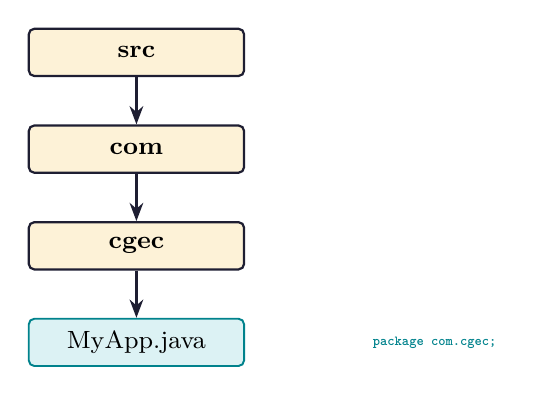
\begin{tikzpicture}[node distance=0.8cm and 1.5cm,
  folder/.style={rectangle, draw=mydark, fill=hdramber, text width=2.5cm,
    align=center, minimum height=0.6cm, font=\small\bfseries, rounded corners=2pt, line width=0.8pt},
  file/.style={rectangle, draw=myteal, fill=hdrteal, text width=2.5cm,
    align=center, minimum height=0.6cm, font=\small, rounded corners=2pt, line width=0.7pt}]

  % Folders
  \node[folder] (src) {src};
  \node[folder, below=0.6cm of src] (com) {com};
  \node[folder, below=0.6cm of com] (cgec) {cgec};
  \node[file, below=0.6cm of cgec] (app) {MyApp.java};

  % Paths
  \draw[arrow] (src) -- (com);
  \draw[arrow] (com) -- (cgec);
  \draw[arrow] (cgec) -- (app);

  % Package statement explanation
  \node[right=of app, font=\tiny\ttfamily\bfseries, color=myteal] {package com.cgec;};
\end{tikzpicture}
\end{tcolorbox}

% ===============================================================================
\section{Access Control Mechanism}
% ===============================================================================

Java uses access modifiers to control visibility of classes, constructors, variables, and methods.

\begin{itemize}[leftmargin=*, itemsep=3.5pt]
  \item \textbf{\texttt{private}:} Visible only within the declaring class. It provides the highest encapsulation.
  \item \textbf{Default (Package-Private):} Visible to all classes in the same package. No keyword is specified.
  \item \textbf{\texttt{protected}:} Visible to all classes in the same package, and to subclasses in different packages.
  \item \textbf{\texttt{public}:} Accessible from any class anywhere in the application.
\end{itemize}

% ===============================================================================
\section{Dynamic Method Lookup}
% ===============================================================================

Dynamic Method Lookup (or Interface-based Dynamic Binding) is the runtime mechanism by which the JVM resolves calls to interface methods.

\begin{tcolorbox}[defbox, title={\textbf{Interface Callbacks}}]
When an interface reference calls a method, the JVM looks up the actual runtime class of the referenced object, retrieves its dynamic method table, and invokes the concrete overridden method. This is the foundation of loose coupling and polymorphic callbacks.
\end{tcolorbox}

\begin{tcolorbox}[tikzbox, title={Interface Callback Mechanism}]
\centering
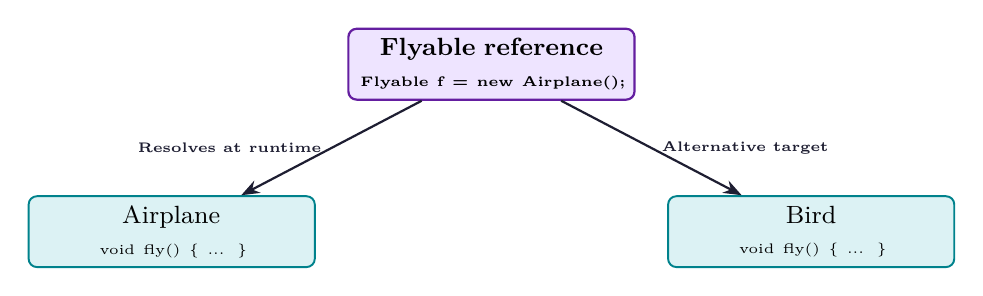
\begin{tikzpicture}[node distance=1.2cm and 2.2cm,
  intf/.style={rectangle, draw=mypurple, fill=hdrpurple, text width=3.4cm,
    align=center, minimum height=0.9cm, font=\small\bfseries, rounded corners=3pt, line width=0.8pt},
  impl/.style={rectangle, draw=myteal, fill=hdrteal, text width=3.4cm,
    align=center, minimum height=0.9cm, font=\small, rounded corners=3pt, line width=0.7pt}]

  % Interface reference
  \node[intf] (ref) {Flyable reference\\{\tiny Flyable f = new Airplane();}};
  
  % Implementing classes
  \node[impl, below left=1.2cm and 0.4cm of ref] (air) {Airplane\\{\tiny void fly() \{ ... \}}};
  \node[impl, below right=1.2cm and 0.4cm of ref] (bird) {Bird\\{\tiny void fly() \{ ... \}}};

  % Paths
  \draw[arrow] (ref) -- (air) node[midway, left, font=\tiny\bfseries] {Resolves at runtime};
  \draw[arrow] (ref) -- (bird) node[midway, right, font=\tiny\bfseries] {Alternative target};
\end{tikzpicture}
\tcbset{after={\color{black}}}
\end{tcolorbox}

\newpage
% ===============================================================================
\begin{center}
  {\large\bfseries\color{myred} Quick Revision --- Module 4}\\[3pt]
  {\small\color{mydark} Interfaces and Packages $|$ OE-EC704A}
\end{center}
\noindent{\color{myred}\rule{\linewidth}{1.2pt}}
\vspace{4pt}

\begin{tcolorbox}[formulabox, title={\textbf{Interface \& Package Declarations}}]
{\renewcommand{\arraystretch}{1.3}%
\begin{tabularx}{\linewidth}{l Y}
\textbf{Concept} & \textbf{Syntax and Example Usage} \\
\hline
Interface Definition & \texttt{interface InterfaceName \{ void methodSignature(); \}} \\
Implementation & \texttt{class ClassName implements InterfaceName \{ ... \}} \\
Default Method & \texttt{default void log() \{ System.out.println("Default Log"); \}} \\
Static Method & \texttt{static int add(int a, int b) \{ return a + b; \}} \\
\hline
\textbf{Packages \& Imports} & \textbf{Core syntax headers} \\
\hline
Package Declaration & \texttt{package com.cgec.webtech; // must be first line} \\
Class Import & \texttt{import java.util.ArrayList;} \\
Wildcard Import & \texttt{import java.util.*;} \\
Static Import & \texttt{import static java.lang.Math.PI;} \\
\end{tabularx}}
\end{tcolorbox}

\begin{tcolorbox}[defbox, title={\textbf{One-Line Definitions}}]
\begin{itemize}[leftmargin=*, itemsep=2pt]
  \item \textbf{Interface:} A reference type declaring method signatures and constants, defining a contract.
  \item \textbf{Package:} A directory structure grouping related classes and interfaces.
  \item \textbf{Default Method:} An interface method containing a default body, declared with the \texttt{default} keyword.
  \item \textbf{Access Modifier:} Keywords controlling the accessibility level of classes and class members.
  \item \textbf{Dynamic Method Lookup:} Runtime resolution of interface method calls based on actual object instance type.
  \item \textbf{Encapsulation:} Bundling class state and behavior while restricting direct access using private.
  \item \textbf{Namespace:} A naming container resolving name conflicts across different components.
  \item \textbf{Multiple Inheritance:} Implementing multiple interfaces to inherit behaviors from multiple sources.
\end{itemize}
\tcbset{after={\color{black}}}
\end{tcolorbox}

\begin{tcolorbox}[exambox, title={\textbf{Frequently Asked / Viva Questions}}]
\begin{enumerate}[leftmargin=*, label=\textbf{Q\arabic*.}, itemsep=5pt]
  \item \Q{Can an interface be instantiated? Why?}
        No. An interface does not have constructors and contains abstract method signatures without implementations, so it cannot represent concrete runtime state.
        
  \item \Q{Why does Java allow multiple inheritance using interfaces but not classes?}
        Classes hold state (instance variables). If a class inherits from multiple parent classes, duplicate variable names cause conflicts. Since interfaces hold no state variables (only constants) and historically had no implementations, there is no duplicate implementation ambiguity.
        
  \item \Q{What is the difference between an Interface and an Abstract Class?}
        An abstract class can contain instance variables (state) and constructors, whereas an interface can only contain public static final constants. A class can extend only one class but implement multiple interfaces.
        
  \item \Q{What are default methods and why were they introduced in Java 8?}
        Default methods have concrete bodies declared with the \texttt{default} keyword inside an interface. They allow adding new methods to interfaces without breaking existing classes that implement the interface.
        
  \item \Q{What is a functional interface?}
        An interface containing exactly one abstract method. It can be annotated with \texttt{@FunctionalInterface} and is used for Lambda expressions (e.g., \texttt{Runnable}, \texttt{Comparable}).
        
  \item \Q{Can we declare an interface method as \texttt{private} or \texttt{protected}?}
        Interface abstract methods must be \texttt{public}. However, starting from Java 9, we can declare \texttt{private} and \texttt{private static} helper methods inside interfaces. \texttt{protected} is never allowed.
        
  \item \Q{What is the default access modifier in an interface?}
        All fields are implicitly \texttt{public static final}. All abstract methods are implicitly \texttt{public abstract}.
        
  \item \Q{What is a static import in Java?}
        A static import allows importing static members (variables and methods) of a class directly (e.g., \texttt{import static java.lang.Math.sqrt;}). This allows invoking them without prepending the class name.
        
  \item \Q{What is the difference between \texttt{package} and \texttt{import} statements?}
        The \texttt{package} statement declares which package/directory the current class belongs to. The \texttt{import} statement tells the compiler where to find other classes referenced in the file.
        
  \item \Q{How does the JVM resolve name conflicts between classes in different imported packages?}
        If a class with the same name exists in two imported packages (e.g., \texttt{java.util.Date} and \texttt{java.sql.Date}), the compiler forces the developer to use the fully qualified class name in code to resolve ambiguity.
\end{enumerate}
\end{tcolorbox}

\begin{tcolorbox}[tikzbox, title={Java Access Modifier Visibility Matrix}]
\centering
{\renewcommand{\arraystretch}{1.45}%
\begin{tabularx}{\linewidth}{|B{2.8cm}|>{\centering\arraybackslash}X|>{\centering\arraybackslash}X|>{\centering\arraybackslash}X|>{\centering\arraybackslash}X|}
\hline
\textbf{Modifier} & \textbf{Same Class} & \textbf{Same Package} & \textbf{Subclass} & \textbf{Everywhere} \\
\hline
\textbf{\texttt{private}} & Yes & No & No & No \\
\hline
\textbf{Default} & Yes & Yes & No & No \\
\hline
\textbf{\texttt{protected}} & Yes & Yes & Yes & No \\
\hline
\textbf{\texttt{public}} & Yes & Yes & Yes & Yes \\
\hline
\end{tabularx}}
\tcbset{after={\color{black}}}
\end{tcolorbox}


% -- Module 5 -----------------------------------------------------------------
\modulestart{5}{Java Exception Handling Mechanism}

\section{Java Exception Handling Mechanism}
% ===============================================================================

An exception is an unwanted or unexpected event that occurs during the execution of a program (at runtime) and disrupts the normal flow of instructions.

\begin{tcolorbox}[defbox, title={\textbf{Exception Handling Goals}}]
The primary goal of exception handling is to prevent runtime program crashes and allow the application to handle errors gracefully, releasing resources and reporting descriptive messages.
\end{tcolorbox}

\begin{tcolorbox}[tikzbox, title={Java Exception Class Hierarchy}]
\centering
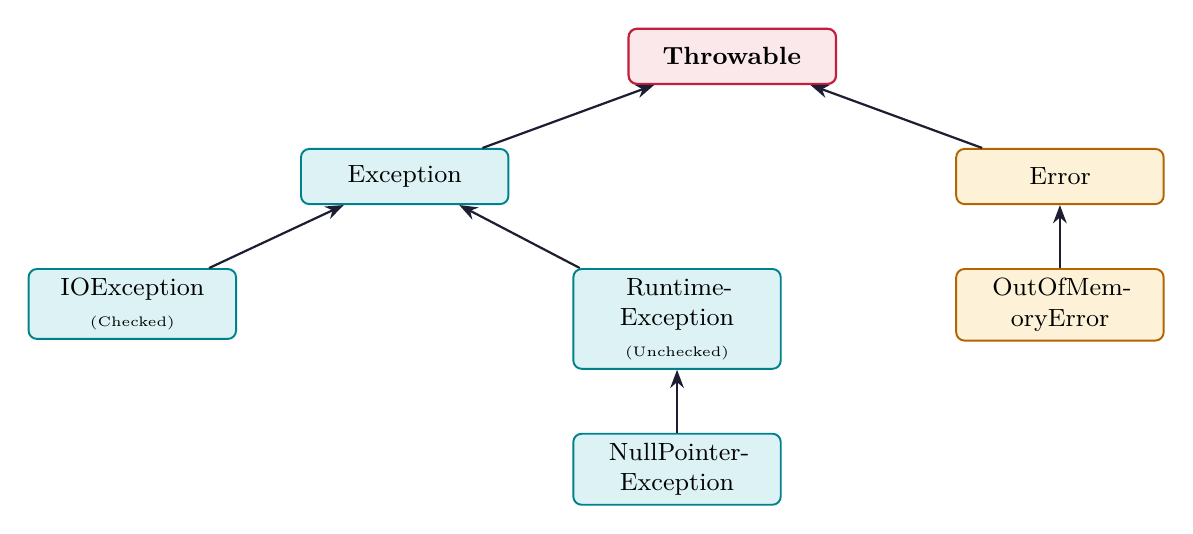
\begin{tikzpicture}[node distance=1.2cm and 1.5cm,
  root/.style={rectangle, draw=myred, fill=hdrred, text width=2.4cm,
    align=center, minimum height=0.7cm, font=\small\bfseries, rounded corners=3pt, line width=0.8pt},
  node/.style={rectangle, draw=myteal, fill=hdrteal, text width=2.4cm,
    align=center, minimum height=0.7cm, font=\small, rounded corners=3pt, line width=0.7pt},
  error/.style={rectangle, draw=myamber, fill=hdramber, text width=2.4cm,
    align=center, minimum height=0.7cm, font=\small, rounded corners=3pt, line width=0.7pt}]

  % Hierarchy Nodes
  \node[root] (throw) {Throwable};
  \node[node, below left=0.8cm and 1.5cm of throw] (ex) {Exception};
  \node[error, below right=0.8cm and 1.5cm of throw] (err) {Error};
  
  \node[node, below left=0.8cm and 0.8cm of ex] (chk) {IOException\\{\tiny (Checked)}};
  \node[node, below right=0.8cm and 0.8cm of ex] (rt) {RuntimeException\\{\tiny (Unchecked)}};
  
  \node[error, below=0.8cm of err] (oome) {OutOfMemoryError};
  \node[node, below=0.8cm of rt] (npe) {NullPointer-\\Exception};

  % Paths
  \draw[arrow] (ex) -- (throw);
  \draw[arrow] (err) -- (throw);
  \draw[arrow] (chk) -- (ex);
  \draw[arrow] (rt) -- (ex);
  \draw[arrow] (npe) -- (rt);
  \draw[arrow] (oome) -- (err);
\end{tikzpicture}
\end{tcolorbox}

\subsection{Throwable Hierarchy}
The root class of the exception hierarchy is \texttt{java.lang.Throwable}. Only objects that are instances of this class (or subclasses) can be thrown by the JVM or the Java \texttt{throw} statement.
\begin{itemize}[leftmargin=*, itemsep=3.5pt]
  \item \textbf{Error:} Extends \texttt{Throwable}. Represents serious problems that a reasonable application should not try to catch (e.g., \texttt{VirtualMachineError}, \texttt{OutOfMemoryError}, \texttt{StackOverflowError}). They represent infrastructure or JVM failures.
  \item \textbf{Exception:} Extends \texttt{Throwable}. Represents conditions that a reasonable application might want to catch and handle.
\end{itemize}

\subsection{Checked vs. Unchecked Exceptions}
\begin{itemize}[leftmargin=*, itemsep=4pt]
  \item \textbf{Checked Exceptions:} Classes that extend \texttt{Exception} but do not extend \texttt{RuntimeException}. They are verified by the compiler at compile-time. The program must handle them using try-catch or declare them using the \texttt{throws} clause (e.g., \texttt{IOException}, \texttt{SQLException}, \texttt{ClassNotFoundException}).
  \item \textbf{Unchecked Exceptions:} Classes that extend \texttt{RuntimeException}. They are not checked by the compiler. They usually result from logical errors or bad program state (e.g., \texttt{NullPointerException}, \texttt{ArithmeticException}, \texttt{ArrayIndexOutOfBoundsException}).
\end{itemize}

% ===============================================================================
\section{Exception Keywords \& Handling Structures}
% ===============================================================================

Java exception handling is managed via five keywords: \texttt{try}, \texttt{catch}, \texttt{finally}, \texttt{throw}, and \texttt{throws}.

\subsection{Try-Catch-Finally Blocks}
\begin{itemize}[leftmargin=*, itemsep=4pt]
  \item \textbf{\texttt{try}:} Surrounds the block of code that might throw an exception. It must be followed by at least one \texttt{catch} block or a \texttt{finally} block.
  \item \textbf{\texttt{catch}:} Defines the exception handler. Multiple catch blocks can follow a single try block, starting from the most specific exception subclass to the most general (superclass).
  \item \textbf{\texttt{finally}:} Executed guaranteed, whether an exception occurs or not, and even if there is a return statement inside try/catch. Used for cleanup tasks like closing resources.
\end{itemize}

\subsection{Throw vs. Throws}
\begin{itemize}[leftmargin=*, itemsep=4.5pt]
  \item \textbf{\texttt{throw}:} Used to explicitly throw an instance of any class extending \texttt{Throwable} from code (e.g., \texttt{throw new ArithmeticException("Divide by zero");}).
  \item \textbf{\texttt{throws}:} Used in method declarations to list the checked exceptions that the method might throw, delegating the responsibility of handling to the caller method (e.g., \texttt{public void read() throws IOException \{ ... \}}).
\end{itemize}

\subsection{Try-with-Resources and the \texttt{AutoCloseable} Interface}
Introduced in Java 7, the try-with-resources statement is a try block declared with one or more resource declarations.
\begin{verbatim}
try (BufferedReader br = new BufferedReader(new FileReader("test.txt"))) {
    System.out.println(br.readLine());
} catch (IOException e) {
    e.printStackTrace();
}
\end{verbatim}
\begin{itemize}[leftmargin=*, itemsep=3.5pt]
  \item Any class declared inside the try parentheses must implement the \texttt{java.lang.AutoCloseable} interface.
  \item The JVM automatically closes these resources when the try block exits, eliminating the need for verbose manual resource-closing logic inside a \texttt{finally} block.
\end{itemize}

\subsection{User-Defined / Custom Exceptions}
Developers can create custom exceptions to represent domain-specific errors.
\begin{itemize}[leftmargin=*, itemsep=3pt]
  \item To create a checked exception, extend the \texttt{java.lang.Exception} class.
  \item To create an unchecked exception, extend the \texttt{java.lang.RuntimeException} class.
\end{itemize}
\begin{verbatim}
class InvalidAgeException extends Exception {
    public InvalidAgeException(String message) {
        super(message);
    }
}
\end{verbatim}

\newpage
% ===============================================================================
\begin{center}
  {\large\bfseries\color{myred} Quick Revision --- Module 5}\\[3pt]
  {\small\color{mydark} Exception Handling $|$ OE-EC704A}
\end{center}
\noindent{\color{myred}\rule{\linewidth}{1.2pt}}
\vspace{4pt}

\begin{tcolorbox}[formulabox, title={\textbf{Exception Handling Code Constructs}}]
{\renewcommand{\arraystretch}{1.3}%
\begin{tabularx}{\linewidth}{l Y}
\textbf{Structure} & \textbf{Syntax and Example Usage} \\
\hline
Try-Catch Block & \texttt{try \{ int val = 10 / 0; \} catch(ArithmeticException e) \{ ... \}} \\
Try-With-Resources & \texttt{try (FileReader fr = new FileReader("file.txt")) \{ ... \}} \\
Method Throws Clause & \texttt{public void load() throws IOException, ClassNotFoundException \{ ... \}} \\
Explicit Throw & \texttt{throw new NullPointerException("Null Reference Encountered");} \\
Custom Exception & \texttt{class CustomException extends RuntimeException \{ CustomException(String m)\{super(m);\} \}} \\
\end{tabularx}}
\tcbset{after={\color{black}}}
\end{tcolorbox}

\begin{tcolorbox}[defbox, title={\textbf{One-Line Definitions}}]
\begin{itemize}[leftmargin=*, itemsep=2pt]
  \item \textbf{Exception:} An event disrupting the normal instruction execution flow.
  \item \textbf{Checked Exception:} An exception subclass checked at compile-time, requiring try-catch or throws.
  \item \textbf{Unchecked Exception:} An exception subclass extending RuntimeException, not checked at compile-time.
  \item \textbf{Error:} A fatal system condition that applications should not attempt to handle.
  \item \textbf{Try Block:} A block enclosing code that might generate a runtime exception.
  \item \textbf{Finally Block:} A block executing guaranteed cleanup actions, running after try-catch completion.
  \item \textbf{Try-with-Resources:} An automatic resource management block closing AutoCloseable targets automatically.
  \item \textbf{AutoCloseable:} Interface defining the \texttt{close()} contract for automatic try-with-resources cleanups.
\end{itemize}
\tcbset{after={\color{black}}}
\end{tcolorbox}

\begin{tcolorbox}[exambox, title={\textbf{Frequently Asked / Viva Questions}}]
\begin{enumerate}[leftmargin=*, label=\textbf{Q\arabic*.}, itemsep=5pt]
  \item \Q{What is the difference between Checked and Unchecked exceptions?}
        Checked exceptions are verified by the compiler at compile-time (e.g., \texttt{IOException}) and must be handled or declared. Unchecked exceptions are RuntimeExceptions (e.g., \texttt{NullPointerException}) and are not compiler-checked.
        
  \item \Q{What is the difference between \texttt{final}, \texttt{finally}, and \texttt{finalize}?}
        \texttt{final} is a keyword making variables unassignable, methods override-protected, and classes inheritance-protected. \texttt{finally} is a block for resource cleanup in exception handling. \texttt{finalize} is a method invoked by the Garbage Collector before object reclamation.
        
  \item \Q{Can we have a try block without a catch block?}
        Yes. A try block can be followed by a \texttt{finally} block instead of a catch block, or it can be a try-with-resources statement which handles closing automatically.
        
  \item \Q{What is Exception Propagation?}
        If an exception is not caught in the method where it occurred, it propagates down the call stack to the calling method. This repeats until it is handled or the JVM terminates the thread.
        
  \item \Q{What is class \texttt{Throwable}? What are its main subclasses?}
        \texttt{Throwable} is the root class of all exceptions and errors in Java. Its main subclasses are \texttt{java.lang.Exception} and \texttt{java.lang.Error}.
        
  \item \Q{How does multi-catch work in Java 7?}
        A single catch block can handle multiple unrelated exceptions using the pipe symbol (e.g., \texttt{catch (IOException | SQLException e)}). The variable \texttt{e} is implicitly final.
        
  \item \Q{What happens if an exception is thrown in a \texttt{finally} block?}
        If an exception is thrown in a finally block, it overrides and suppresses any active exception previously thrown in the try or catch blocks, unless handled internally.
        
  \item \Q{Why should more specific catch blocks be declared before general ones?}
        Java matches catch blocks from top to bottom. If a general exception catch block (like \texttt{Exception}) is placed first, it will catch all subclass exceptions, making subsequent specific catch blocks unreachable and causing compile errors.
        
  \item \Q{What is class \texttt{AutoCloseable}?}
        It is a functional interface introduced in Java 7 containing a single method: \texttt{void close() throws Exception}. Classes implementing this interface are automatically closed in a try-with-resources construct.
        
  \item \Q{Is it possible to throw a checked exception from static initializer block?}
        No. A static initializer block runs when the class is loaded and cannot throw checked exceptions since there is no calling method to catch or declare them.
\end{enumerate}
\end{tcolorbox}

\begin{tcolorbox}[tikzbox, title={Checked vs. Unchecked Exception Comparison}]
\centering
{\renewcommand{\arraystretch}{1.45}%
\begin{tabularx}{\linewidth}{|B{3.2cm}|Y|Y|}
\hline
\textbf{Metric} & \textbf{Checked Exception} & \textbf{Unchecked Exception} \\
\hline
\textbf{Compilation Check} & Checked at compile-time by compiler. & Ignored by compiler during build. \\
\hline
\textbf{Handling Rule} & Must use try-catch or declare throws. & Optional to handle; fix logic instead. \\
\hline
\textbf{Base Class} & Directly extends \texttt{java.lang.Exception}. & Extends \texttt{java.lang.RuntimeException}. \\
\hline
\textbf{Root Cause} & External environment issues (I/O, network). & Program logical errors (null checks, math). \\
\hline
\end{tabularx}}
\tcbset{after={\color{black}}}
\end{tcolorbox}


% -- Module 6 -----------------------------------------------------------------
\modulestart{6}{String Basics and Immutability}

\section{String Basics and Immutability}
% ===============================================================================

In Java, strings are represented by the \texttt{String} class inside the \texttt{java.lang} package. 

\begin{tcolorbox}[defbox, title={\textbf{String Immutability Concept}}]
Java String objects are \textbf{immutable}, meaning their values cannot be changed once they are created in memory. Any modification operation (like concatenation or case conversion) does not alter the original string; instead, it returns a reference to a completely new String object.
\end{tcolorbox}

\subsection{String Constant Pool (SCP)}
To save memory and increase performance, JVM maintains a special memory area inside the heap called the \textbf{String Constant Pool (SCP)}.
\begin{itemize}[leftmargin=*, itemsep=3.5pt]
  \item \textbf{Literal Allocation:} When a string is created using a literal (e.g., \texttt{String s1 = "Java";}), JVM first checks the SCP. If the string is already present, it returns the existing reference. Otherwise, it allocates a new string in the pool.
  \item \textbf{New Object Allocation:} Using the \texttt{new} keyword (e.g., \texttt{String s2 = new String("Java");}) bypasses pool checking and creates a new object in the general heap space, which references the literal value in the SCP.
\end{itemize}

\begin{tcolorbox}[tikzbox, title={String Memory References: General Heap vs. String Constant Pool (SCP)}]
\centering
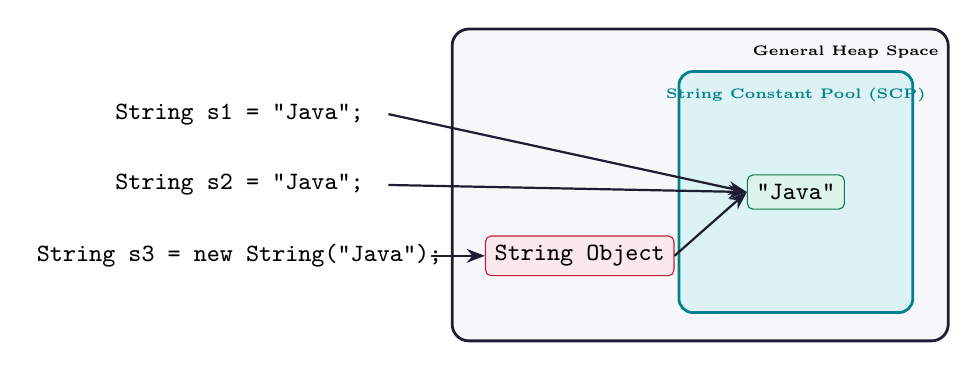
\begin{tikzpicture}[scale=0.9]
  % Stack variables
  \node (s1) at (-4, 2) {\small\texttt{String s1 = "Java";}};
  \node (s2) at (-4, 1) {\small\texttt{String s2 = "Java";}};
  \node (s3) at (-4, 0) {\small\texttt{String s3 = new String("Java");}};

  % General Heap Boundary
  \draw[draw=mydark, fill=mygray, line width=1pt, rounded corners=6pt] (-1,-1.2) rectangle (6,3.2);
  \node[anchor=north east, font=\tiny\bfseries] at (6,3.1) {General Heap Space};

  % SCP Boundary inside Heap
  \draw[draw=myteal, fill=hdrteal, line width=1pt, rounded corners=5pt] (2.2,-0.8) rectangle (5.5,2.6);
  \node[anchor=north, font=\tiny\bfseries, color=myteal] at (3.85,2.5) {String Constant Pool (SCP)};

  % String value inside SCP
  \node[draw=mygreen, fill=hdrgreen, rounded corners=2pt, font=\small\ttfamily] (java_literal) at (3.85, 0.9) {"Java"};

  % Heap object
  \node[draw=myred, fill=hdrred, rounded corners=2pt, font=\small\ttfamily] (heap_obj) at (0.8, 0) {String Object};

  % Connections
  \draw[arrow] (-1.9, 2) -- (java_literal.west);
  \draw[arrow] (-1.9, 1) -- (java_literal.west);
  \draw[arrow] (-1.3, 0) -- (heap_obj.west);
  \draw[arrow] (heap_obj.east) -- (java_literal.west);
\end{tikzpicture}
\end{tcolorbox}

% ===============================================================================
\section{String vs. StringBuffer}
% ===============================================================================

When a program performs frequent modifications to character sequences, using the immutable \texttt{String} class generates high amounts of garbage references. Java provides \texttt{StringBuffer} to resolve this.

\par\noindent
{\renewcommand{\arraystretch}{1.5}%
\begin{tabularx}{\linewidth}{|B{3.2cm}|Y|Y|}
\hline
\textbf{Metric} & \textbf{String Class} & \textbf{StringBuffer Class} \\
\hline
\textbf{Mutability} & Immutable (read-only). & Mutable (can modify in-place). \\
\hline
\textbf{Performance} & Slower for modifications. & Fast and memory efficient for loops. \\
\hline
\textbf{Thread Safety} & Naturally thread-safe. & Thread-safe (methods are synchronized). \\
\hline
\textbf{Memory Allocation} & Allocations inside the SCP or Heap. & Allocated strictly in the general Heap. \\
\hline
\end{tabularx}}

% ===============================================================================
\section{Constructors and Core Operations}
% ===============================================================================

\subsection{String Constructors}
\begin{itemize}[leftmargin=*, itemsep=3pt]
  \item \texttt{String()}: Initializes a newly created, empty String object.
  \item \texttt{String(char[] chars)}: Allocates a new String from an array of characters.
  \item \texttt{String(String original)}: Creates a copy of the argument string.
\end{itemize}

\subsection{Core String Operations}
\par\noindent
{\renewcommand{\arraystretch}{1.45}%
\begin{tabularx}{\linewidth}{|B{2.8cm}|B{4.5cm}|Y|}
\hline
\textbf{Operation} & \textbf{Method Signature} & \textbf{Functional Description} \\
\hline
\textbf{Extraction} & \texttt{char charAt(int index)} & Returns the character at the specified index. \\
                    & \texttt{int length()} & Returns the character count. \\
\hline
\textbf{Comparison} & \texttt{boolean equals(Object obj)} & Value-based comparison for character equality. \\
                    & \texttt{int compareTo(String another)} & Lexicographically compares two strings (returns difference). \\
\hline
\textbf{Searching}  & \texttt{int indexOf(String str)} & Returns the index of the first occurrence. \\
                    & \texttt{boolean contains(CharSequence s)} & Returns true if the string matches the pattern. \\
\hline
\textbf{Modifying}  & \texttt{String substring(int start, int end)} & Returns characters from start (incl.) to end (excl.). \\
                    & \texttt{String trim()} & Removes leading and trailing whitespace. \\
\hline
\end{tabularx}}

% ===============================================================================
\section{Utility Conversions}
% ===============================================================================

Java provides two major methods to perform conversions to strings:
\begin{itemize}[leftmargin=*, itemsep=3.5pt]
  \item \textbf{\texttt{toString()} Method:} Defined in the root \texttt{Object} class. Every Java class inherits it and can override it to provide a custom string representation of the object's fields.
  \item \textbf{\texttt{String.valueOf()} Static Method:} Overloaded methods to convert primitive data types (like \texttt{int}, \texttt{double}, \texttt{boolean}) or objects into string representations. If an object is passed, it returns \texttt{obj.toString()} or \texttt{"null"} safely if the reference is null.
\end{itemize}

% ===============================================================================
\section{StringBuffer Operations}
% ===============================================================================

\texttt{StringBuffer} maintains a growable character buffer, defaulting to 16 characters of extra capacity.
\begin{itemize}[leftmargin=*, itemsep=3.5pt]
  \item \textbf{\texttt{append()}:} Appends data to the end of the buffer.
  \item \textbf{\texttt{insert()}:} Inserts data at a specified index.
  \item \textbf{\texttt{reverse()}:} Reverses the sequence of characters in-place.
  \item \textbf{Capacity vs. Length:} \texttt{length()} returns the actual number of characters stored, while \texttt{capacity()} returns the total allocated buffer space.
\end{itemize}

\newpage
% ===============================================================================
\begin{center}
  {\large\bfseries\color{myred} Quick Revision --- Module 6}\\[3pt]
  {\small\color{mydark} String Handling $|$ OE-EC704A}
\end{center}
\noindent{\color{myred}\rule{\linewidth}{1.2pt}}
\vspace{4pt}

\begin{tcolorbox}[formulabox, title={\textbf{String \& StringBuffer Syntax}}]
{\renewcommand{\arraystretch}{1.3}%
\begin{tabularx}{\linewidth}{l Y}
\textbf{Operation} & \textbf{Syntax and Example Usage} \\
\hline
Literal Assignment & \texttt{String s1 = "Biraj"; // Allocated in SCP} \\
Object Constructor & \texttt{String s2 = new String("Biraj"); // Heap object reference} \\
Character Extraction & \texttt{char c = s1.charAt(2); // 'r'} \\
Substring Extraction & \texttt{String sub = s1.substring(1, 3); // "ir"} \\
\hline
\textbf{StringBuffer Operations} & \textbf{Mutable buffer syntax} \\
\hline
Declaration & \texttt{StringBuffer sb = new StringBuffer("CGE");} \\
Append Operation & \texttt{sb.append("C"); // sb becomes "CGEC"} \\
Insert Operation & \texttt{sb.insert(3, "-"); // sb becomes "CGE-C"} \\
In-place Reverse & \texttt{sb.reverse(); // sb becomes "C-EGC"} \\
\end{tabularx}}
\end{tcolorbox}

\begin{tcolorbox}[defbox, title={\textbf{One-Line Definitions}}]
\begin{itemize}[leftmargin=*, itemsep=2pt]
  \item \textbf{Immutability:} State constraint preventing modification of heap values after initial allocation.
  \item \textbf{String Constant Pool:} A cached region in Java heap memory storing unique string literals.
  \item \textbf{StringBuffer:} A thread-safe, synchronized, mutable character sequence class.
  \item \textbf{StringBuilder:} A non-synchronized, fast, mutable character sequence class.
  \item \textbf{equals():} Overridden method in String checking value-based character equality.
  \item \textbf{== Operator:} Operator checking whether two reference variables point to the same memory address.
  \item \textbf{valueOf():} Static String utility method converting primitives and objects to strings.
  \item \textbf{toString():} Standard Object method returning class representation details as a String.
\end{itemize}
\tcbset{after={\color{black}}}
\end{tcolorbox}

\begin{tcolorbox}[exambox, title={\textbf{Frequently Asked / Viva Questions}}]
\begin{enumerate}[leftmargin=*, label=\textbf{Q\arabic*.}, itemsep=5pt]
  \item \Q{Why are String objects immutable in Java?}
        To enable String Constant Pool caching (saving heap memory), ensure thread-safety, and prevent security vulnerabilities (since connection strings and file paths cannot be altered).
        
  \item \Q{What is the difference between \texttt{equals()} and \texttt{==} when comparing Strings?}
        \texttt{==} compares reference equality (whether variables point to the exact same object reference). The \texttt{equals()} method checks value equality (whether character sequences are identical).
        
  \item \Q{How many objects are created in the statement: \texttt{String s = new String("Hello");}?}
        Two objects. One literal object is placed in the String Constant Pool (if not already present), and a second String object is created in the general heap space.
        
  \item \Q{What does the method \texttt{intern()} do?}
        It returns the canonical representation of the string from the String Constant Pool. If the pool already contains the string, it returns its reference; otherwise, it adds the string to the pool and returns the reference.
        
  \item \Q{What is the difference between \texttt{StringBuffer} and \texttt{StringBuilder}?}
        Both are mutable classes. \texttt{StringBuffer} is thread-safe and has synchronized methods, causing high performance overhead. \texttt{StringBuilder} is not synchronized, making it faster and preferred for single-threaded applications.
        
  \item \Q{What is the default capacity of a \texttt{StringBuffer}? How does it increase?}
        The default initial capacity is 16. When the buffer capacity is exceeded, it grows automatically using the formula: $\text{New Capacity} = (\text{Old Capacity} \times 2) + 2$.
        
  \item \Q{Can we override the static method \texttt{valueOf()} in custom classes?}
        No. Static methods belong to the class scope and are resolved statically during compilation. They cannot be overridden in subclasses. Custom classes override \texttt{toString()} instead.
        
  \item \Q{What does the method \texttt{compareTo()} return?}
        It returns $0$ if strings are equal, a negative integer if the current string is lexicographically smaller than the argument, and a positive integer if it is larger.
        
  \item \Q{Why does \texttt{System.out.println(obj)} invoke the \texttt{toString()} method?}
        The print streams implicitly check if the argument is an object. If yes, it calls \texttt{String.valueOf(obj)}, which internally invokes \texttt{obj.toString()} to get a printable string.
        
  \item \Q{What is the purpose of the \texttt{trim()} method in the String class?}
        It returns a copy of the string with all leading and trailing whitespaces (characters with Unicode code point less than or equal to \texttt{'U+0020'}) removed.
\end{enumerate}
\end{tcolorbox}

\begin{tcolorbox}[tikzbox, title={Comparison: String vs. StringBuffer vs. StringBuilder}]
\centering
{\renewcommand{\arraystretch}{1.45}%
\begin{tabularx}{\linewidth}{|B{2.8cm}|Y|Y|Y|}
\hline
\textbf{Metric} & \textbf{String} & \textbf{StringBuffer} & \textbf{StringBuilder} \\
\hline
\textbf{Mutability} & Immutable. & Mutable. & Mutable. \\
\hline
\textbf{Thread Safety} & Yes (due to immutability). & Yes (synchronized methods). & No (non-synchronized). \\
\hline
\textbf{Performance} & Slowest for edits. & Slower (lock overhead). & Fastest. \\
\hline
\textbf{Introduced in} & Java 1.0 & Java 1.0 & Java 1.5 \\
\hline
\end{tabularx}}
\tcbset{after={\color{black}}}
\end{tcolorbox}


% -- Module 7 -----------------------------------------------------------------
\modulestart{7}{Java I/O Stream Basics}

\section{Java I/O Stream Basics}
% ===============================================================================

An Input/Output (I/O) Stream represents an abstraction of a data source (e.g., keyboard, file) or destination (e.g., console, network socket).

\begin{tcolorbox}[defbox, title={\textbf{Stream Concept}}]
A \textbf{Stream} is a continuous sequence of data bytes. Input streams are used to read data from a source, and Output streams are used to write data to a target.
\end{tcolorbox}

\subsection{Byte Stream vs. Character Stream}
Java's I/O library operates on two primary categories of streams:
\begin{itemize}[leftmargin=*, itemsep=3.5pt]
  \item \textbf{Byte Streams:} Process data as raw 8-bit bytes. They are suitable for binary data (images, sound, zip files).
  \item \textbf{Character Streams:} Process data as 16-bit Unicode characters. They handle translation of text encoding models automatically.
\end{itemize}

\begin{tcolorbox}[tikzbox, title={Java Stream Hierarchy}]
\centering
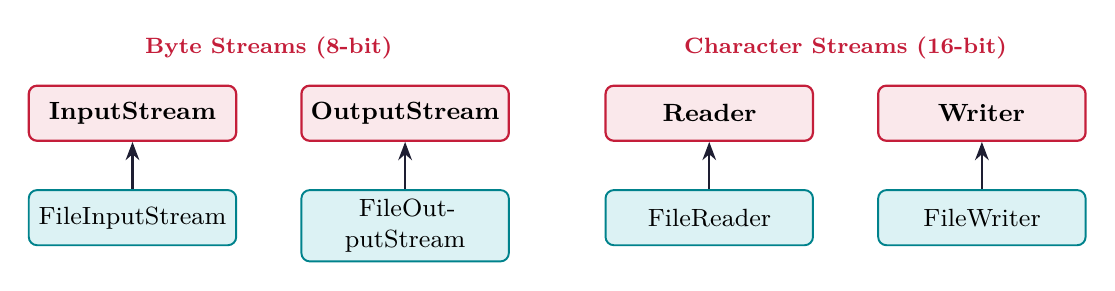
\begin{tikzpicture}[node distance=0.8cm and 1.2cm,
  base/.style={rectangle, draw=myred, fill=hdrred, text width=2.4cm,
    align=center, minimum height=0.7cm, font=\small\bfseries, rounded corners=3pt, line width=0.8pt},
  sub/.style={rectangle, draw=myteal, fill=hdrteal, text width=2.4cm,
    align=center, minimum height=0.7cm, font=\small, rounded corners=3pt, line width=0.7pt}]

  % Byte Streams
  \node[base] (is) {InputStream};
  \node[sub, below=0.6cm of is] (fis) {FileInputStream};
  \draw[arrow] (fis) -- (is);
  
  \node[base, right=0.8cm of is] (os) {OutputStream};
  \node[sub, below=0.6cm of os] (fos) {FileOutputStream};
  \draw[arrow] (fos) -- (os);

  % Character Streams
  \node[base, right=1.2cm of os] (rd) {Reader};
  \node[sub, below=0.6cm of rd] (fr) {FileReader};
  \draw[arrow] (fr) -- (rd);
  
  \node[base, right=0.8cm of rd] (wr) {Writer};
  \node[sub, below=0.6cm of wr] (fw) {FileWriter};
  \draw[arrow] (fw) -- (wr);

  % Labels
  \node[above=0.2cm of $(is.north)!0.5!(os.north)$, font=\footnotesize\bfseries, color=myred] {Byte Streams (8-bit)};
  \node[above=0.2cm of $(rd.north)!0.5!(wr.north)$, font=\footnotesize\bfseries, color=myred] {Character Streams (16-bit)};
\end{tikzpicture}
\end{tcolorbox}

% ===============================================================================
\section{Console I/O Operations}
% ===============================================================================

Java represents console streams using three static variables declared in the \texttt{System} class:
\begin{itemize}[leftmargin=*, itemsep=3pt]
  \item \textbf{\texttt{System.in}:} Standard Input Stream (type \texttt{InputStream}), mapped to keyboard input.
  \item \textbf{\texttt{System.out}:} Standard Output Stream (type \texttt{PrintStream}), mapped to console output.
  \item \textbf{\texttt{System.err}:} Standard Error Stream (type \texttt{PrintStream}), mapped to console error output.
\end{itemize}

\subsection{Reading Console via BufferedReader}
Because \texttt{System.in} is a byte stream, we wrap it in a character stream (\texttt{InputStreamReader}) and pass it to a \texttt{BufferedReader} to enable line-by-line reading:
\begin{verbatim}
BufferedReader br = new BufferedReader(new InputStreamReader(System.in));
System.out.print("Enter your name: ");
String name = br.readLine();
\end{verbatim}

\subsection{Reading Console via Scanner}
The \texttt{java.util.Scanner} class parses primitives and strings using regular expressions:
\begin{verbatim}
Scanner sc = new Scanner(System.in);
System.out.print("Enter an integer: ");
int value = sc.nextInt();
\end{verbatim}

% ===============================================================================
\section{File I/O Operations}
% ===============================================================================

\subsection{FileInputStream and FileOutputStream}
Used to read and write raw bytes from/to a file on disk:
\begin{verbatim}
// Copying a binary file byte-by-byte
try (FileInputStream fis = new FileInputStream("input.jpg");
     FileOutputStream fos = new FileOutputStream("output.jpg")) {
    int byteData;
    while ((byteData = fis.read()) != -1) {
        fos.write(byteData);
    }
} catch (IOException e) {
    e.printStackTrace();
}
\end{verbatim}

\subsection{FileReader and FileWriter}
Used to read and write character text data from/to files on disk:
\begin{verbatim}
try (FileReader fr = new FileReader("file.txt");
     FileWriter fw = new FileWriter("copy.txt")) {
    int charData;
    while ((charData = fr.read()) != -1) {
        fw.write(charData);
    }
} catch (IOException e) {
    e.printStackTrace();
}
\end{verbatim}

\subsection{Buffered Stream Wrapper Pattern}
Disk I/O requests are expensive. To improve performance, we wrap base stream classes inside buffered wrapper classes:
\begin{itemize}[leftmargin=*, itemsep=3.5pt]
  \item \textbf{\texttt{BufferedReader}:} Wraps around a \texttt{Reader} (e.g., \texttt{FileReader}) to buffer characters, providing a highly efficient \texttt{readLine()} method.
  \item \textbf{\texttt{BufferedWriter}:} Wraps around a \texttt{Writer} to buffer written characters, writing to disk only when the buffer is full or when \texttt{flush()} is invoked.
\end{itemize}

\newpage
% ===============================================================================
\begin{center}
  {\large\bfseries\color{myred} Quick Revision --- Module 7}\\[3pt]
  {\small\color{mydark} Java I/O Streams $|$ OE-EC704A}
\end{center}
\noindent{\color{myred}\rule{\linewidth}{1.2pt}}
\vspace{4pt}

\begin{tcolorbox}[formulabox, title={\textbf{Java I/O Stream Syntax}}]
{\renewcommand{\arraystretch}{1.3}%
\begin{tabularx}{\linewidth}{l Y}
\textbf{Construct} & \textbf{Syntax and Example Usage} \\
\hline
Console BufferedReader & \texttt{BufferedReader br = new BufferedReader(new InputStreamReader(System.in));} \\
Console Scanner & \texttt{Scanner sc = new Scanner(System.in); int val = sc.nextInt();} \\
File Reader (Text) & \texttt{FileReader fr = new FileReader("input.txt"); int c = fr.read();} \\
File Writer (Text) & \texttt{FileWriter fw = new FileWriter("output.txt"); fw.write("Hello");} \\
File Byte Input & \texttt{FileInputStream fis = new FileInputStream("in.dat"); fis.read();} \\
Buffered Writer Wrapper & \texttt{BufferedWriter bw = new BufferedWriter(new FileWriter("out.txt"));} \\
\end{tabularx}}
\end{tcolorbox}

\begin{tcolorbox}[defbox, title={\textbf{One-Line Definitions}}]
\begin{itemize}[leftmargin=*, itemsep=2pt]
  \item \textbf{Stream:} A logical abstraction of a continuous sequence of data bytes.
  \item \textbf{Byte Stream:} Stream processing raw 8-bit binary data units.
  \item \textbf{Character Stream:} Stream processing 16-bit Unicode character data units.
  \item \textbf{InputStreamReader:} A bridge class converting byte streams into character streams.
  \item \textbf{BufferedReader:} A character stream wrapper that caches characters in memory to reduce disk calls.
  \item \textbf{Scanner:} A text scanner utility class parsing primitives using token delimiters.
  \item \textbf{System.in:} Static instance of InputStream mapped to the client keyboard.
  \item \textbf{System.out:} Static instance of PrintStream mapped to the standard console output.
\end{itemize}
\tcbset{after={\color{black}}}
\end{tcolorbox}

\begin{tcolorbox}[exambox, title={\textbf{Frequently Asked / Viva Questions}}]
\begin{enumerate}[leftmargin=*, label=\textbf{Q\arabic*.}, itemsep=5pt]
  \item \Q{What is the difference between Byte Streams and Character Streams?}
        Byte streams read/write data as 8-bit bytes (base classes: \texttt{InputStream}, \texttt{OutputStream}), ideal for binary files. Character streams read/write data as 16-bit Unicode characters (base classes: \texttt{Reader}, \texttt{Writer}), ideal for text files.
        
  \item \Q{Why do we wrap a \texttt{FileReader} inside a \texttt{BufferedReader}?}
        Reading directly from disk is slow. Wrapping in a \texttt{BufferedReader} caches character chunks in memory, reducing physical disk reads, and exposes the convenient \texttt{readLine()} method.
        
  \item \Q{What is the purpose of the \texttt{InputStreamReader} class?}
        It acts as a bridge, converting a byte stream (like \texttt{System.in}) into a character stream, translating bytes into characters using the default system charset.
        
  \item \Q{What is the difference between \texttt{PrintStream} and \texttt{PrintWriter}?}
        \texttt{PrintStream} is a byte stream class handling 8-bit output (like \texttt{System.out}). \texttt{PrintWriter} is a character stream class handling 16-bit Unicode character output.
        
  \item \Q{What does the method \texttt{flush()} do in output streams?}
        It forces the output stream to write any cached buffered bytes/characters immediately to the destination device (like the disk file), emptying the local memory buffer.
        
  \item \Q{What is the default buffer size of a \texttt{BufferedReader}?}
        The default buffer size is 8192 characters (8 KB), which is large enough to handle most typical text file read sizes efficiently.
        
  \item \Q{How does the \texttt{Scanner} class handle delimiters?}
        By default, the \texttt{Scanner} class uses whitespace (spaces, tabs, newlines) as the token delimiter. This can be customized using the \texttt{useDelimiter()} method.
        
  \item \Q{What is the difference between \texttt{read()} method of \texttt{InputStream} and \texttt{Reader}?}
        \texttt{InputStream.read()} reads a single byte and returns it as an integer ($0$ to $255$). \texttt{Reader.read()} reads a single Unicode character and returns it as an integer ($0$ to $65535$). Both return $-1$ when reaching EOF.
        
  \item \Q{What checked exception is commonly thrown during file operations?}
        \texttt{java.io.IOException} and its subclass \texttt{java.io.FileNotFoundException}. They must be explicitly caught or declared using a \texttt{throws} clause.
        
  \item \Q{What are the standard console stream fields inside the \texttt{System} class?}
        \texttt{System.in} (standard input - \texttt{InputStream}), \texttt{System.out} (standard output - \texttt{PrintStream}), and \texttt{System.err} (standard error - \texttt{PrintStream}).
\end{enumerate}
\end{tcolorbox}

\begin{tcolorbox}[tikzbox, title={Comparison: Reader/Writer vs. InputStream/OutputStream}]
\centering
{\renewcommand{\arraystretch}{1.45}%
\begin{tabularx}{\linewidth}{|B{3.2cm}|Y|Y|}
\hline
\textbf{Metric} & \textbf{Reader / Writer Hierarchy} & \textbf{InputStream / OutputStream Hierarchy} \\
\hline
\textbf{Data Unit} & 16-bit Unicode character unit. & 8-bit raw byte unit. \\
\hline
\textbf{Primary Target} & Text documents and strings. & Images, sound, ZIP, raw binary data. \\
\hline
\textbf{Root Packages} & Lives inside \texttt{java.io} & Lives inside \texttt{java.io} \\
\hline
\textbf{Default EOF value} & Returns $-1$ at stream end. & Returns $-1$ at stream end. \\
\hline
\end{tabularx}}
\tcbset{after={\color{black}}}
\end{tcolorbox}


% -- Module 8 -----------------------------------------------------------------
\modulestart{8}{Java Collections Framework Overview}

\section{Java Collections Framework Overview}
% ===============================================================================

The Collections Framework, declared inside the \texttt{java.util} package, provides a unified architecture to store and manipulate a group of objects.

\begin{tcolorbox}[defbox, title={\textbf{Core Design Benefits}}]
\begin{itemize}[leftmargin=*, itemsep=3pt]
  \item Reduces programming effort by providing standard data structures.
  \item Boosts speed and quality via high-performance, optimized implementations.
  \item Promotes software reuse by offering polymorphic operations.
\end{itemize}
\end{tcolorbox}

\subsection{Core Interfaces}
The framework is structured hierarchically around a set of core interfaces:
\begin{itemize}[leftmargin=*, itemsep=4pt]
  \item \textbf{\texttt{Collection}:} The root interface defining basic operations (size, add, remove, clear).
  \item \textbf{\texttt{List}:} Extends \texttt{Collection}. Represents an ordered sequence of elements that can contain duplicates. Supports index-based access.
  \item \textbf{\texttt{Set}:} Extends \texttt{Collection}. A collection that cannot contain duplicate elements, modeling mathematical sets.
  \item \textbf{\texttt{Queue}:} Extends \texttt{Collection}. Designed to hold elements prior to processing (typically FIFO).
\end{itemize}

% ===============================================================================
\section{ArrayList vs. LinkedList}
% ===============================================================================

\par\noindent
{\renewcommand{\arraystretch}{1.5}%
\begin{tabularx}{\linewidth}{|B{3.2cm}|Y|Y|}
\hline
\textbf{Metric} & \textbf{\texttt{ArrayList}} & \textbf{\texttt{LinkedList}} \\
\hline
\textbf{Internal Structure} & Dynamically resizing array. & Doubly linked list nodes. \\
\hline
\textbf{Access Time} & $O(1)$ random access (index-based). & $O(n)$ search access (sequential traverse). \\
\hline
\textbf{Insertion/Deletion} & $O(n)$ (requires element shifts). & $O(1)$ if pointer is located. \\
\hline
\textbf{Memory Overhead} & Low (only stores elements). & Higher (stores element and prev/next links). \\
\hline
\end{tabularx}}

\begin{tcolorbox}[tikzbox, title={ArrayList vs. LinkedList Memory Layout}]
\centering
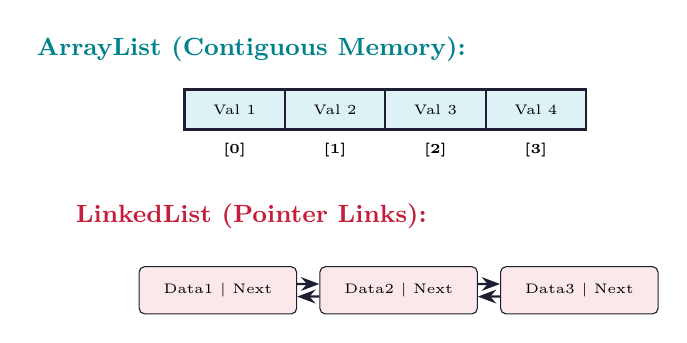
\begin{tikzpicture}[scale=0.85]
  % ArrayList
  \node[font=\small\bfseries, color=myteal] at (1,2) {ArrayList (Contiguous Memory):};
  \draw[draw=mydark, fill=hdrteal, line width=1pt] (0,0.8) rectangle (6,1.4);
  \foreach \x in {1.5, 3.0, 4.5} {
    \draw[line] (\x, 0.8) -- (\x, 1.4);
  }
  \node[font=\tiny] at (0.75, 1.1) {Val 1};
  \node[font=\tiny] at (2.25, 1.1) {Val 2};
  \node[font=\tiny] at (3.75, 1.1) {Val 3};
  \node[font=\tiny] at (5.25, 1.1) {Val 4};

  \node[font=\tiny\bfseries] at (0.75, 0.5) {[0]};
  \node[font=\tiny\bfseries] at (2.25, 0.5) {[1]};
  \node[font=\tiny\bfseries] at (3.75, 0.5) {[2]};
  \node[font=\tiny\bfseries] at (5.25, 0.5) {[3]};

  % LinkedList
  \node[font=\small\bfseries, color=myred] at (1,-0.5) {LinkedList (Pointer Links):};
  
  \node[draw=mydark, fill=hdrred, minimum width=2.0cm, minimum height=0.6cm, rounded corners=2pt] (n1) at (0.5,-1.6) {\tiny Data1 | Next};
  \node[draw=mydark, fill=hdrred, minimum width=2.0cm, minimum height=0.6cm, rounded corners=2pt] (n2) at (3.2,-1.6) {\tiny Data2 | Next};
  \node[draw=mydark, fill=hdrred, minimum width=2.0cm, minimum height=0.6cm, rounded corners=2pt] (n3) at (5.9,-1.6) {\tiny Data3 | Next};

  \draw[arrow, transform canvas={yshift=0.08cm}] (n1) -- (n2);
  \draw[arrow, transform canvas={yshift=-0.08cm}] (n2) -- (n1);
  \draw[arrow, transform canvas={yshift=0.08cm}] (n2) -- (n3);
  \draw[arrow, transform canvas={yshift=-0.08cm}] (n3) -- (n2);
\end{tikzpicture}
\tcbset{after={\color{black}}}
\end{tcolorbox}

% ===============================================================================
\section{Accessing and Iterating Collections}
% ===============================================================================

Java provides two primary mechanisms to traverse through collection elements:

\subsection{The Iterator Interface}
An iterator provides sequential access to collection elements. It is retrieved using \texttt{iterator()} method on any Collection object.
\begin{verbatim}
ArrayList<String> list = new ArrayList<>();
list.add("Java");
list.add("HTML");

Iterator<String> itr = list.iterator();
while (itr.hasNext()) {
    String element = itr.next();
    System.out.println(element);
}
\end{verbatim}
\begin{itemize}[leftmargin=*, itemsep=3.5pt]
  \item \textbf{Methods:} \texttt{hasNext()} (returns true if more elements exist), \texttt{next()} (returns next element), and \texttt{remove()} (removes current element safely during iteration).
  \item \textbf{Fail-Fast Behavior:} Iterators on standard collections like ArrayList throw a \texttt{ConcurrentModificationException} if the collection is structurally modified (add/remove) outside the iterator's own methods during iteration.
\end{itemize}

\subsection{The For-Each Statement}
Introduced in Java 5, the enhanced \texttt{for} loop (for-each) provides a cleaner syntax to iterate over arrays and collections:
\begin{verbatim}
for (String element : list) {
    System.out.println(element);
}
\end{verbatim}
Internally, the compiler translates this syntax into standard Iterator-based code for objects implementing the \texttt{java.lang.Iterable} interface.

\newpage
% ===============================================================================
\begin{center}
  {\large\bfseries\color{myred} Quick Revision --- Module 8}\\[3pt]
  {\small\color{mydark} Java Utility package - Collections $|$ OE-EC704A}
\end{center}
\noindent{\color{myred}\rule{\linewidth}{1.2pt}}
\vspace{4pt}

\begin{tcolorbox}[formulabox, title={\textbf{Collection Syntax}}]
{\renewcommand{\arraystretch}{1.3}%
\begin{tabularx}{\linewidth}{l Y}
\textbf{Construct} & \textbf{Syntax and Example Usage} \\
\hline
ArrayList Declaration & \texttt{ArrayList<String> list = new ArrayList<String>();} \\
ArrayList Insert & \texttt{list.add("Java"); list.add(1, "CSS"); // inserts at index 1} \\
LinkedList Declaration & \texttt{LinkedList<Integer> lList = new LinkedList<>();} \\
Iterator Traversal & \texttt{Iterator<String> itr = list.iterator(); while(itr.hasNext()) \{ ... \}} \\
For-Each Loop & \texttt{for (String str : list) \{ System.out.println(str); \}} \\
\end{tabularx}}
\end{tcolorbox}

\begin{tcolorbox}[defbox, title={\textbf{One-Line Definitions}}]
\begin{itemize}[leftmargin=*, itemsep=2pt]
  \item \textbf{Collections Framework:} Architecture of interfaces and classes for grouping multiple objects.
  \item \textbf{ArrayList:} Resizable-array implementation of the List interface, backing elements contiguously.
  \item \textbf{LinkedList:} Doubly-linked node implementation of the List and Deque interfaces.
  \item \textbf{Iterator:} Object traversal cursor enabling forward traversal and safe element removals.
  \item \textbf{Fail-Fast Iterator:} Iterator throwing exception immediately if collection structure changes during loop.
  \item \textbf{Iterable:} Interface indicating target object can be traversed using enhanced for-each.
  \item \textbf{Generics:} Compiler feature ensuring type-safety in collections (e.g., \texttt{ArrayList<String>}).
  \item \textbf{Auto-boxing:} Implicit compiler conversion between primitives and their wrapper classes.
\end{itemize}
\tcbset{after={\color{black}}}
\end{tcolorbox}

\begin{tcolorbox}[exambox, title={\textbf{Frequently Asked / Viva Questions}}]
\begin{enumerate}[leftmargin=*, label=\textbf{Q\arabic*.}, itemsep=5pt]
  \item \Q{What is the difference between \texttt{ArrayList} and \texttt{Vector}?}
        \texttt{ArrayList} is non-synchronized, fast, and not thread-safe. \texttt{Vector} is synchronized, has thread-safe methods, and carries significant execution overhead.
        
  \item \Q{Why does a \texttt{LinkedList} consume more memory than an \texttt{ArrayList}?}
        An \texttt{ArrayList} stores elements contiguously inside a backing array. A \texttt{LinkedList} wraps each element inside a node object that also holds reference addresses for the previous and next nodes.
        
  \item \Q{What is fail-fast behavior in collections?}
        It is a JVM runtime validation that throws a \texttt{ConcurrentModificationException} if a collection is modified structurally (elements added or deleted) while an active iterator is traversing it.
        
  \item \Q{How does ArrayList grow its internal array capacity?}
        When an element is added and the array is full, ArrayList allocates a new array and copies elements. Starting from Java 10, it increases capacity by roughly $50\%$ ($\text{New Capacity} = \text{Old Capacity} + (\text{Old Capacity} \gg 1)$).
        
  \item \Q{What is the purpose of the \texttt{Iterable} interface?}
        It is the superinterface of the \texttt{Collection} interface. Implementing \texttt{Iterable} requires the class to return an \texttt{Iterator}, allowing instances to be used in the enhanced for-each loop.
        
  \item \Q{Can we store primitive data types (like \texttt{int}, \texttt{char}) inside collections?}
        No, collections only store object references. However, Java handles this automatically using \textbf{Autoboxing}, which converts primitives to their wrapper objects (e.g., \texttt{int} to \texttt{Integer}) when inserted.
        
  \item \Q{What is the difference between \texttt{Iterator} and \texttt{ListIterator}?}
        \texttt{Iterator} can traverse any Collection in a forward direction. \texttt{ListIterator} can only traverse Lists, but supports bidirectional traversal (forward and backward) and element modifications.
        
  \item \Q{Which List implementation is preferred for frequent search operations?}
        \texttt{ArrayList} is preferred because it supports $O(1)$ constant time lookup via index-based access, whereas \texttt{LinkedList} requires $O(n)$ linear traversal.
        
  \item \Q{Which List implementation is preferred for frequent insertions at the beginning of the list?}
        \texttt{LinkedList} is preferred. Inserting at the beginning requires only updating two node pointers ($O(1)$), whereas \texttt{ArrayList} requires shifting all existing elements, taking $O(n)$ time.
        
  \item \Q{What is the difference between \texttt{List} and \texttt{Set} interfaces?}
        A \texttt{List} maintains insertion order and can contain duplicate elements. A \texttt{Set} is unordered and cannot contain duplicate elements.
\end{enumerate}
\end{tcolorbox}

\begin{tcolorbox}[tikzbox, title={ArrayList vs. LinkedList operations complexity}]
\centering
{\renewcommand{\arraystretch}{1.45}%
\begin{tabularx}{\linewidth}{|B{3.2cm}|Y|Y|}
\hline
\textbf{Operation} & \textbf{ArrayList} & \textbf{LinkedList} \\
\hline
\textbf{Get by Index} & $O(1)$ constant time. & $O(n)$ linear traversal. \\
\hline
\textbf{Insert/Delete (Start)} & $O(n)$ shift overhead. & $O(1)$ pointer change. \\
\hline
\textbf{Insert/Delete (End)} & $O(1)$ amortized. & $O(1)$ tail reference update. \\
\hline
\textbf{Memory consumption} & Low (consecutive slots). & High (two references per node). \\
\hline
\end{tabularx}}
\tcbset{after={\color{black}}}
\\
\end{tcolorbox}


% -- Module 9 -----------------------------------------------------------------
\modulestart{9}{Introduction to Applets}

\section{Introduction to Applets}
% ===============================================================================

An applet is a specialized Java program designed to be embedded within an HTML web page and executed on a client machine inside a web browser sandbox.

\begin{tcolorbox}[defbox, title={\textbf{Applet Security Sandbox}}]
To prevent malicious code execution on client machines, applets run under strict security constraints:
\begin{itemize}[leftmargin=*, itemsep=3pt]
  \item Applets cannot read or write files on the local client disk.
  \item Applets cannot communicate with any host except the one they were downloaded from.
  \item Applets cannot execute local system commands or load native runtime libraries.
\end{itemize}
\end{tcolorbox}

\subsection{Applet Lifecycle \& Execution}
An applet inherits from \texttt{java.applet.Applet} and does not contain a \texttt{main()} method. Instead, its execution is controlled by the browser or the Java Applet Viewer tool through five lifecycle callback methods:
\begin{itemize}[leftmargin=*, itemsep=4pt]
  \item \textbf{\texttt{init()}:} Invoked once when the applet is first loaded to perform initialization (e.g., setting up GUI components, reading parameters).
  \item \textbf{\texttt{start()}:} Invoked after \texttt{init()} or whenever the user returns to the web page containing the applet. Used to start or resume execution threads.
  \item \textbf{\texttt{paint(Graphics g)}:} Invoked when the applet window needs to be redrawn (e.g., first display, resizing, or revealing). It uses the \texttt{java.awt.Graphics} object.
  \item \textbf{\texttt{stop()}:} Invoked when the user navigates away from the page, pausing background threads to save CPU cycles.
  \item \textbf{\texttt{destroy()}:} Invoked once before unloading the applet completely to free up system resources.
\end{itemize}

\begin{tcolorbox}[tikzbox, title={Applet Life Cycle State Transitions}]
\centering
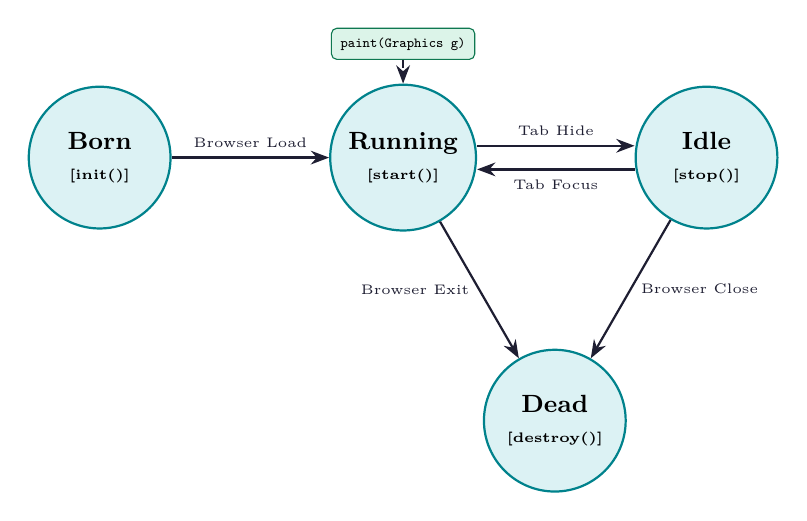
\begin{tikzpicture}[node distance=1.3cm and 2.0cm,
  state/.style={circle, draw=myteal, fill=hdrteal, minimum size=1.8cm,
    align=center, font=\small\bfseries, line width=0.8pt},
  act/.style={rectangle, draw=myamber, fill=hdramber, minimum height=0.6cm,
    font=\tiny, rounded corners=2pt, line width=0.6pt}]

  % States
  \node[state] (born) {Born\\{\tiny [init()]}};
  \node[state, right=2.0cm of born] (run) {Running\\{\tiny [start()]}};
  \node[state, right=2.0cm of run] (idle) {Idle\\{\tiny [stop()]}};
  \node[state, below=1.5cm of $(run.south)!0.5!(idle.south)$] (dead) {Dead\\{\tiny [destroy()]}};

  % Paths
  \draw[arrow] (born) -- (run) node[midway, above, font=\tiny] {Browser Load};
  \draw[arrow, transform canvas={yshift=0.15cm}] (run) -- (idle) node[midway, above, font=\tiny] {Tab Hide};
  \draw[arrow, transform canvas={yshift=-0.15cm}] (idle) -- (run) node[midway, below, font=\tiny] {Tab Focus};
  \draw[arrow] (idle) -- (dead) node[midway, right, font=\tiny] {Browser Close};
  \draw[arrow] (run) -- (dead) node[midway, left, font=\tiny] {Browser Exit};

  % Paint Call
  \node[draw=mygreen, fill=hdrgreen, rounded corners=2pt, above=0.3cm of run, font=\tiny] (pnt) {\texttt{paint(Graphics g)}};
  \draw[arrow, dashed] (pnt) -- (run);
\end{tikzpicture}
\end{tcolorbox}

% ===============================================================================
\section{Applet Display and Status Window}
% ===============================================================================

Since \texttt{Applet} extends the AWT \texttt{Panel} container class, it supports all standard component styling methods:
\begin{itemize}[leftmargin=*, itemsep=3.5pt]
  \item \textbf{\texttt{setBackground(Color c)} / \texttt{setForeground(Color c)}:} Configures the background canvas color and text drawing color.
  \item \textbf{\texttt{showStatus(String msg)}:} Displays the specified text message in the status bar of the browser or Applet Viewer, providing interactive feedback.
\end{itemize}

% ===============================================================================
\section{HTML Embedding and Parameter Passing}
% ===============================================================================

Applets are embedded in web pages using the HTML \texttt{<applet>} tag. 

\subsection{HTML Applet Tag Syntax}
\begin{verbatim}
<applet code="MyApplet.class" width="300" height="200" codebase="bin/">
    <param name="fontName" value="Courier">
    <param name="fontSize" value="14">
    Alt Text: Applets are not supported by your browser.
</applet>
\end{verbatim}
\begin{itemize}[leftmargin=*, itemsep=3pt]
  \item \textbf{\texttt{code}:} Specifies the compiled applet class filename.
  \item \textbf{\texttt{width} \& \texttt{height}:} Declares the size of the applet execution area on the web page.
  \item \textbf{\texttt{codebase}:} Specifies the base directory URL containing the class bytecode.
\end{itemize}

\subsection{Parameter Retrieval via getParameter()}
The \texttt{<param>} tags allow passing configuration parameters to the applet during load time. Inside the applet's \texttt{init()} method, their values are read as Strings:
\begin{verbatim}
String fontStr = getParameter("fontName"); // Returns "Courier"
int size = Integer.parseInt(getParameter("fontSize")); // Parses 14
\end{verbatim}

\subsection{getCodeBase() and getDocumentBase()}
To locate resources (images, audio clips) dynamically:
\begin{itemize}[leftmargin=*, itemsep=3.5pt]
  \item \textbf{\texttt{getCodeBase()}:} Returns the base URL of the directory containing the compiled class bytecode.
  \item \textbf{\texttt{getDocumentBase()}:} Returns the URL of the HTML document embedding the applet.
\end{itemize}

\newpage
% ===============================================================================
\begin{center}
  {\large\bfseries\color{myred} Quick Revision --- Module 9}\\[3pt]
  {\small\color{mydark} Java Applets $|$ OE-EC704A}
\end{center}
\noindent{\color{myred}\rule{\linewidth}{1.2pt}}
\vspace{4pt}

\begin{tcolorbox}[formulabox, title={\textbf{HTML Applet Tag \& Parameters}}]
{\renewcommand{\arraystretch}{1.3}%
\begin{tabularx}{\linewidth}{l Y}
\textbf{Construct} & \textbf{Syntax and Example Usage} \\
\hline
HTML Applet Tag & \texttt{<applet code="MyApp.class" width="400" height="300"></applet>} \\
Param Value Tag & \texttt{<param name="bgColor" value="red">} \\
Parameter Query & \texttt{String val = getParameter("bgColor");} \\
Status Output & \texttt{showStatus("Applet loading completed successfully");} \\
Get Code URL & \texttt{URL codeBaseUrl = getCodeBase();} \\
Get Doc URL & \texttt{URL docBaseUrl = getDocumentBase();} \\
\end{tabularx}}
\end{tcolorbox}

\begin{tcolorbox}[defbox, title={\textbf{One-Line Definitions}}]
\begin{itemize}[leftmargin=*, itemsep=2pt]
  \item \textbf{Applet:} A client-side Java program executed inside a browser container sandbox.
  \item \textbf{Sandbox:} A secure runtime environment preventing unauthorized access to client resources.
  \item \textbf{init():} The first applet lifecycle method called once to initialize variables and UI.
  \item \textbf{paint():} AWT component method redrawing text and graphics on the applet canvas.
  \item \textbf{getParameter():} Applet method retrieving parameter values defined in HTML.
  \item \textbf{getCodeBase():} Applet method returning the directory URL containing the class file.
  \item \textbf{getDocumentBase():} Applet method returning the URL of the hosting HTML document.
  \item \textbf{AppletViewer:} A JDK utility tool designed to test and execute Java applets without a browser.
\end{itemize}
\tcbset{after={\color{black}}}
\end{tcolorbox}

\begin{tcolorbox}[exambox, title={\textbf{Frequently Asked / Viva Questions}}]
\begin{enumerate}[leftmargin=*, label=\textbf{Q\arabic*.}, itemsep=5pt]
  \item \Q{Which class does every Java Applet extend? Which package contains it?}
        Every Applet extends \texttt{java.applet.Applet} (or \texttt{javax.swing.JApplet} for Swing). The class resides inside the \texttt{java.applet} package.
        
  \item \Q{Why does an applet not contain a \texttt{main()} method?}
        Applets do not run as standalone applications. They are executed by a web browser container, which handles loading and calls their lifecycle methods.
        
  \item \Q{What is the difference between \texttt{init()} and \texttt{start()} methods?}
        \texttt{init()} is called once when the applet is first loaded to handle initialization. \texttt{start()} is called every time the user visits or returns to the page.
        
  \item \Q{What is the purpose of the \texttt{paint(Graphics g)} method? Who calls it?}
        The \texttt{paint()} method renders the applet graphics (text, lines, shapes) on the screen. It is called by the browser JVM when the applet first displays or needs redrawing.
        
  \item \Q{How do you pass parameters from HTML to an Applet?}
        Using the \texttt{<param>} tag inside the \texttt{<applet>} tag in HTML, and querying it in the applet using the \texttt{getParameter(String name)} method.
        
  \item \Q{What is the difference between \texttt{getCodeBase()} and \texttt{getDocumentBase()}?}
        \texttt{getCodeBase()} returns the URL of the directory containing the applet's compiled class files. \texttt{getDocumentBase()} returns the URL of the HTML document embedding the applet.
        
  \item \Q{What is the security sandbox model in applets?}
        The sandbox restricts applets to prevent access to the client filesystem, executing external processes, or making network connections to hosts other than the source server.
        
  \item \Q{Can an applet load native libraries using \texttt{System.loadLibrary()}?}
        No. Under the default security policy sandbox, applets are prohibited from loading native dynamic libraries to prevent unsafe pointer manipulations on the host.
        
  \item \Q{What is the difference between local applets and remote applets?}
        Local applets are stored and executed on the same local computer without network access. Remote applets are downloaded from a remote web server over the network and executed locally.
        
  \item \Q{Why are Java Applets deprecated in modern web development?}
        They require browser plugins (NPAPI) that pose major security risks. Modern browsers have disabled plugin support in favor of HTML5, CSS3, and JavaScript standards.
\end{enumerate}
\end{tcolorbox}

\begin{tcolorbox}[tikzbox, title={Applet Lifecycle Methods Transition Matrix}]
\centering
{\renewcommand{\arraystretch}{1.45}%
\begin{tabularx}{\linewidth}{|B{3.0cm}|Y|Y|}
\hline
\textbf{Method} & \textbf{Invocation Frequency} & \textbf{Primary Purpose} \\
\hline
\textbf{\texttt{init()}} & Invoked once when first loaded. & Initializes variables, loads fonts, images, and GUI elements. \\
\hline
\textbf{\texttt{start()}} & Invoked on load and page returns. & Resumes applet execution, starts animations or threads. \\
\hline
\textbf{\texttt{paint()}} & Invoked on display and redraw requests. & Renders text, shapes, and images to the screen coordinate system. \\
\hline
\textbf{\texttt{stop()}} & Invoked on page exit or tab switch. & Suspends threads, pauses animations to save CPU resources. \\
\hline
\textbf{\texttt{destroy()}} & Invoked once before unloading. & Reclaims resources, kills threads, and cleans up memory. \\
\hline
\end{tabularx}}
\tcbset{after={\color{black}}}
\end{tcolorbox}


% -- Module 10 -----------------------------------------------------------------
\modulestart{10}{Delegation Event Model}

\section{Delegation Event Model}
% ===============================================================================

Java event handling is built on the \textbf{Delegation Event Model}, which separates user interface elements from the logical event processing code.

\begin{tcolorbox}[defbox, title={\textbf{Core Model Components}}]
\begin{itemize}[leftmargin=*, itemsep=3pt]
  \item \textbf{Event Source:} The GUI component that generates the event when acted upon (e.g., \texttt{Button}, \texttt{TextField}).
  \item \textbf{Event Object:} An object encapsulating details of the state change (e.g., \texttt{ActionEvent}, \texttt{MouseEvent}).
  \item \textbf{Event Listener:} An interface defining callback methods to receive and process specific events.
\end{itemize}
\end{tcolorbox}

\begin{tcolorbox}[tikzbox, title={Delegation Event Model Architecture}]
\centering
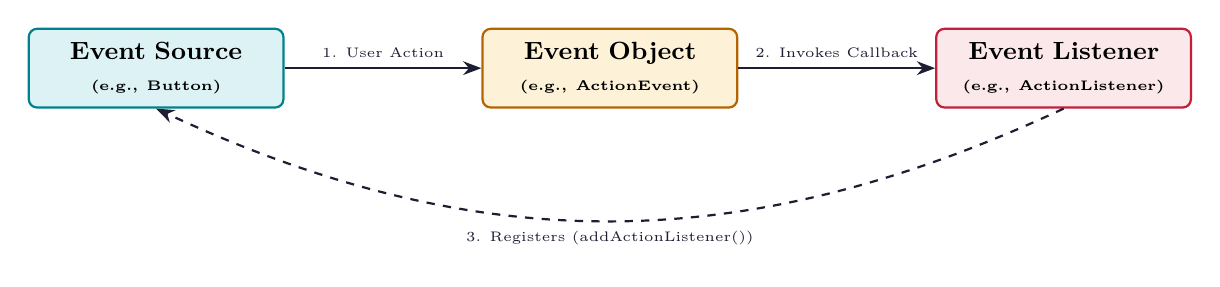
\begin{tikzpicture}[node distance=1.5cm and 2.5cm,
  source/.style={rectangle, draw=myteal, fill=hdrteal, text width=3.0cm,
    align=center, minimum height=1.0cm, font=\small\bfseries, rounded corners=3pt, line width=0.8pt},
  evt/.style={rectangle, draw=myamber, fill=hdramber, text width=3.0cm,
    align=center, minimum height=1.0cm, font=\small\bfseries, rounded corners=3pt, line width=0.8pt},
  listener/.style={rectangle, draw=myred, fill=hdrred, text width=3.0cm,
    align=center, minimum height=1.0cm, font=\small\bfseries, rounded corners=3pt, line width=0.8pt}]

  % Nodes
  \node[source] (src) {Event Source\\{\tiny (e.g., Button)}};
  \node[evt, right=of src] (obj) {Event Object\\{\tiny (e.g., ActionEvent)}};
  \node[listener, right=of obj] (lis) {Event Listener\\{\tiny (e.g., ActionListener)}};

  % Paths
  \draw[arrow] (src) -- (obj) node[midway, above, font=\tiny] {1. User Action};
  \draw[arrow] (obj) -- (lis) node[midway, above, font=\tiny] {2. Invokes Callback};
  
  % Registration path
  \draw[arrow, dashed, bend left=25] (lis.south) to node[midway, below, font=\tiny] {3. Registers (addActionListener())} (src.south);
\end{tikzpicture}
\end{tcolorbox}

\subsection{Common Event Classes \& Listeners}
\par\noindent
{\renewcommand{\arraystretch}{1.45}%
\begin{tabularx}{\linewidth}{|B{3.2cm}|B{4.5cm}|Y|}
\hline
\textbf{Event Source} & \textbf{Event Class} & \textbf{Listener Interface} \\
\hline
\texttt{Button, TextField} & \texttt{ActionEvent} & \texttt{ActionListener} \\
\hline
\texttt{Component} & \texttt{MouseEvent} & \texttt{MouseListener, MouseMotionListener} \\
\hline
\texttt{Component} & \texttt{KeyEvent} & \texttt{KeyListener} \\
\hline
\texttt{Frame, Window} & \texttt{WindowEvent} & \texttt{WindowListener} \\
\hline
\end{tabularx}}

% ===============================================================================
\section{Adapter Classes}
% ===============================================================================

An event listener interface may declare multiple abstract methods. For example, \texttt{WindowListener} has seven methods. Implementing the interface directly forces the developer to write empty method bodies for all seven.

\begin{tcolorbox}[defbox, title={\textbf{Adapter Class Pattern}}]
An \textbf{Adapter Class} is a convenience class that implements a listener interface with empty body definitions. By extending the adapter class (e.g., extending \texttt{WindowAdapter}), you only need to override the specific methods you require.
\end{tcolorbox}

% ===============================================================================
\section{Inner and Anonymous Classes}
% ===============================================================================

To register listeners cleanly without polluting the outer class namespace, Java developers utilize nested class patterns:
\begin{itemize}[leftmargin=*, itemsep=3.5pt]
  \item \textbf{Inner Classes:} Define a private class inside the AWT frame that implements the listener, accessing the frame's components directly.
  \item \textbf{Anonymous Inner Classes:} Define an inline implementation of the listener/adapter class without naming it:
\end{itemize}
\begin{verbatim}
btn.addActionListener(new ActionListener() {
    @Override
    public void actionPerformed(ActionEvent e) {
        System.out.println("Button Clicked!");
    }
});
\end{verbatim}

% ===============================================================================
\section{AWT Controls}
% ===============================================================================

The Abstract Window Toolkit (AWT) provides platform-dependent heavyweight user interface controls:
\begin{itemize}[leftmargin=*, itemsep=3.5pt]
  \item \textbf{\texttt{Label}:} Displays a single line of read-only text.
  \item \textbf{\texttt{Button}:} A clickable control that generates action events.
  \item \textbf{\texttt{TextField} / \texttt{TextArea}:} Single-line and multi-line text input fields.
  \item \textbf{\texttt{Checkbox} / \texttt{Choice}:} Selection controls representing boolean states and drop-down lists.
\end{itemize}

\begin{tcolorbox}[tikzbox, title={AWT Component Class Hierarchy}]
\centering
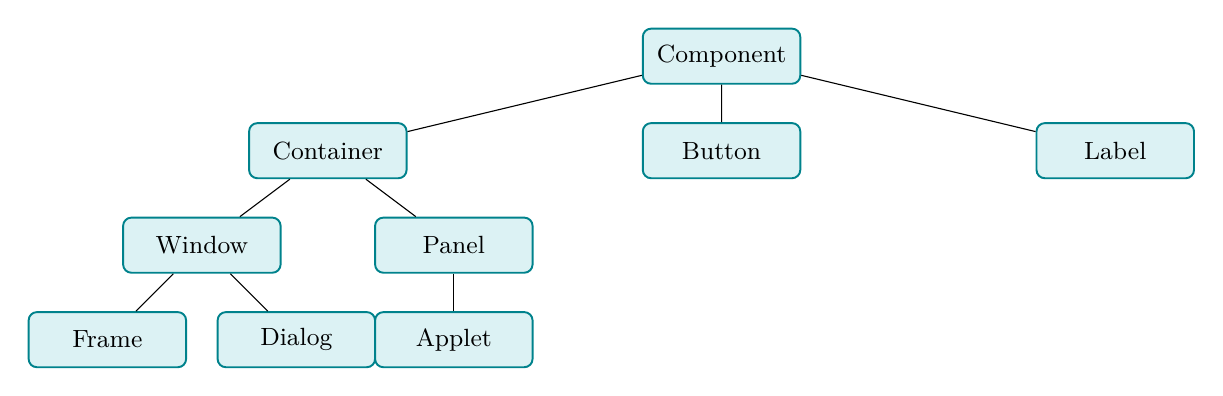
\begin{tikzpicture}[
  level 1/.style={sibling distance=5cm, level distance=1.2cm},
  level 2/.style={sibling distance=3.2cm, level distance=1.2cm},
  level 3/.style={sibling distance=2.4cm, level distance=1.2cm},
  node/.style={rectangle, draw=myteal, fill=hdrteal, minimum height=0.7cm, minimum width=2.0cm, font=\small, rounded corners=3pt, align=center, line width=0.7pt}
]
  \node[node] {Component}
    child { node[node] {Container}
      child { node[node] {Window}
        child { node[node] {Frame} }
        child { node[node] {Dialog} }
      }
      child { node[node] {Panel}
        child { node[node] {Applet} }
      }
    }
    child { node[node] {Button} }
    child { node[node] {Label} };
\end{tikzpicture}
\end{tcolorbox}

% ===============================================================================
\section{Layout Managers}
% ===============================================================================

Layout managers coordinate the sizing and spatial arrangement of components inside a container:
\begin{itemize}[leftmargin=*, itemsep=3.5pt]
  \item \textbf{\texttt{FlowLayout}:} Default for \texttt{Panel} and \texttt{Applet}. Places components in a single line, wrapping left-to-right, top-to-bottom.
  \item \textbf{\texttt{BorderLayout}:} Default for \texttt{Frame} and \texttt{Window}. Divides space into five geographical regions: \texttt{NORTH}, \texttt{SOUTH}, \texttt{EAST}, \texttt{WEST}, and \texttt{CENTER}.
  \item \textbf{\texttt{GridLayout}:} Places components in a uniform grid of equal-sized rows and columns.
\end{itemize}

\newpage
% ===============================================================================
\begin{center}
  {\large\bfseries\color{myred} Quick Revision --- Module 10}\\[3pt]
  {\small\color{mydark} Event Handling \& AWT $|$ OE-EC704A}
\end{center}
\noindent{\color{myred}\rule{\linewidth}{1.2pt}}
\vspace{4pt}

\begin{tcolorbox}[formulabox, title={\textbf{Event \& Layout Syntax}}]
{\renewcommand{\arraystretch}{1.3}%
\begin{tabularx}{\linewidth}{l Y}
\textbf{Construct} & \textbf{Syntax and Example Usage} \\
\hline
Register Action Listener & \texttt{btn.addActionListener(listenerObj);} \\
Anonymous Inner Handler & \texttt{btn.addActionListener(new ActionListener() \{ ... \});} \\
Set Frame Layout & \texttt{frame.setLayout(new BorderLayout());} \\
Add Component Layout & \texttt{frame.add(btn, BorderLayout.CENTER);} \\
Window Closing Adapter & \texttt{f.addWindowListener(new WindowAdapter()\{...WindowClosing...\});} \\
AWT Frame Init & \texttt{Frame f = new Frame("Title"); f.setSize(300, 300); f.setVisible(true);} \\
\end{tabularx}}
\tcbset{after={\color{black}}}
\end{tcolorbox}

\begin{tcolorbox}[defbox, title={\textbf{One-Line Definitions}}]
\begin{itemize}[leftmargin=*, itemsep=2pt]
  \item \textbf{Delegation Event Model:} Framework routing UI events from sources to registered listener objects.
  \item \textbf{Event Source:} GUI control generating event objects on user state changes.
  \item \textbf{Event Listener:} Interface declaring abstract event handler callback operations.
  \item \textbf{Adapter Class:} Convenience class providing empty implementations of listener methods.
  \item \textbf{Heavyweight Control:} A UI component bound to and rendered by a native OS peer window.
  \item \textbf{AWT:} Heavyweight platform-dependent Java GUI framework package.
  \item \textbf{Layout Manager:} Object interface deciding component sizing and layouts within containers.
  \item \textbf{Anonymous Inner Class:} Unnamed class declared and instantiated inline at usage point.
\end{itemize}
\tcbset{after={\color{black}}}
\end{tcolorbox}

\begin{tcolorbox}[exambox, title={\textbf{Frequently Asked / Viva Questions}}]
\begin{enumerate}[leftmargin=*, label=\textbf{Q\arabic*.}, itemsep=5pt]
  \item \Q{How does the Delegation Event Model work?}
        An event source (like a button) generates an event object when interacted with, and delegates processing to one or more registered listener objects by invoking their callback methods.
        
  \item \Q{What is the purpose of Adapter classes in AWT event handling?}
        They simplify listener implementations. Implementing interfaces like \texttt{WindowListener} requires writing empty overrides for all methods. Extending \texttt{WindowAdapter} allows overriding only the required methods.
        
  \item \Q{Why are AWT controls referred to as heavyweight components?}
        AWT controls are coupled to the underlying operating system. Each AWT component is associated with a native peer window, consuming significant OS resources.
        
  \item \Q{What is the difference between AWT and Swing?}
        AWT is platform-dependent and uses heavyweight OS peer rendering. Swing is platform-independent, lightweight, written entirely in Java, and supports a pluggable look-and-feel.
        
  \item \Q{How does FlowLayout arrange components? What is its default alignment?}
        FlowLayout arranges components in a single line from left to right. When it runs out of space, it wraps them to the next line. Its default alignment is centered.
        
  \item \Q{What layout manager is default for Frame? Panel?}
        The default layout manager for a \texttt{Frame} is \texttt{BorderLayout}. The default layout manager for a \texttt{Panel} (and \texttt{Applet}) is \texttt{FlowLayout}.
        
  \item \Q{Which listener interface is used to handle button clicks? Text changes?}
        Button clicks generate ActionEvents and are handled by the \texttt{ActionListener} interface. Text changes in a TextField generate TextEvents, handled by the \texttt{TextListener} interface.
        
  \item \Q{How many regions does a BorderLayout have? What happens if no region is specified?}
        Five regions: North, South, East, West, and Center. If no region is specified when adding a component, it is added to the \texttt{Center} region by default.
        
  \item \Q{Why is an anonymous inner class useful in event handling?}
        It allows declaring and instantiating a listener class inline right where it is registered, keeping code localized and avoiding cluttering the outer class with simple single-method handlers.
        
  \item \Q{How can you close an AWT Frame window when the close button is clicked?}
        By registering a WindowListener (or extending WindowAdapter) and calling \texttt{System.exit(0)} or \texttt{dispose()} inside the overridden \texttt{windowClosing(WindowEvent e)} method.
\end{enumerate}
\end{tcolorbox}

\begin{tcolorbox}[tikzbox, title={Comparison: AWT vs. Swing}]
\centering
{\renewcommand{\arraystretch}{1.45}%
\begin{tabularx}{\linewidth}{|B{3.2cm}|Y|Y|}
\hline
\textbf{Metric} & \textbf{AWT (Heavyweight)} & \textbf{Swing (Lightweight)} \\
\hline
\textbf{Rendering Engine} & OS Native Peer controls. & Painted in Java bytecode. \\
\hline
\textbf{Platform Styling} & Inconsistent look-and-feel. & Uniform style across OS targets. \\
\hline
\textbf{Class Packages} & Lives in \texttt{java.awt.*} & Lives in \texttt{javax.swing.*} \\
\hline
\textbf{GUI Speed} & Slightly faster (OS optimized). & Slightly slower (Java painted). \\
\hline
\end{tabularx}}
\tcbset{after={\color{black}}}
\end{tcolorbox}


\end{document}
